\documentclass{beamer}
\usepackage{booktabs}
\usepackage{ragged2e}
\usepackage{hyperref}
\hypersetup{
    colorlinks=true,
    linkcolor=blue,
    urlcolor=blue,
}
\usetheme{Hannover}
\graphicspath{{../report/figures/}}

\title[]{EPL448 Data Mining Project: Predicting Prices for Used Cars}
\author[]{Andreas Hadjoullis\\Julios Fotiou}
\institute[]{Department of Computer Science \\ University of Cyprus}
\date[]{\today}

\begin{document}

\begin{frame}
        \titlepage
\end{frame}

\begin{frame}{Outline}
        \tableofcontents
\end{frame}

\section{Introduction}
\begin{frame}{Introduction}
        \begin{itemize}
                \item The used car market is huge and rapidly changing. Pricing
                        a used car correctly is crucial for both sellers and
                        buyers.
                \item \textbf{Dataset:} Our dataset initially contained 371,528
                        rows and 21 columns, sourced from \href{https://www.kaggle.com/datasets/thedevastator/uncovering-factors-that-affect-used-car-prices/data}{Kaggle}.
                \item \textbf{Regression Problem:} Accurately predict the selling price of
                        a used car based on its features (brand, model, year,
                        gearbox, etc.).
                \item \textbf{Objectives:}
                        \begin{itemize}
                                \item Explore and analyze the dataset.
                                \item Engineer features and preprocess data.
                                \item Build and evaluate predictive models.
                        \end{itemize}
                \item \textbf{Challenges:} Presence of outliers, irrelevant
                        features, and highly skewed price distribution.
        \end{itemize}
\end{frame}

% Exploratory Data Analysis
\section{Exploratory Data Analysis}
\begin{frame}{Exploratory Data Analysis}
\scriptsize % or \footnotesize
We have the following features:
\vspace{0.5em}

\begin{columns}[t] % Align columns at the top
    \column{0.33\textwidth}
    \textbf{Numerical} \\
    \begin{itemize}
            \item price (\textbf{target})
        \item powerPS
        \item kilometer
        \item monthRegistration
        \item yearOfRegistration
        \item nrOfPictures
        \item postalCode
    \end{itemize}

    \column{0.33\textwidth}
    \textbf{Categorical} \\
    \begin{itemize}
        \item index
        \item name
        \item seller
        \item offerType
        \item abtest
        \item vehicleType
        \item gearbox
        \item model
        \item fuelType
        \item brand
        \item notRepairedDamage
    \end{itemize}

    \column{0.33\textwidth}
    \textbf{Date} \\
    \begin{itemize}
        \item dateCrawled
        \item dateCreated
        \item lastSeen
    \end{itemize}
\end{columns}
\end{frame}

\begin{frame}{Exploratory Data Analysis}
        \begin{itemize}
                \item Kept only rows with realistic prices (€~1,000–200,000) for
                        effective modeling. After removal we remain with
                        288,023 rows.
                \item \texttt{offerType} and \texttt{seller} each had two
                        categories, but one category dominated almost entirely
                        (the minority category had only a handful of rows).
                \item \texttt{nrOfPictures} had only a single unique value for
                        all entries.
                \item These columns were removed as they provided no useful
                        information for prediction.
        \end{itemize}
\end{frame}

\begin{frame}{Target Variable Analysis}
%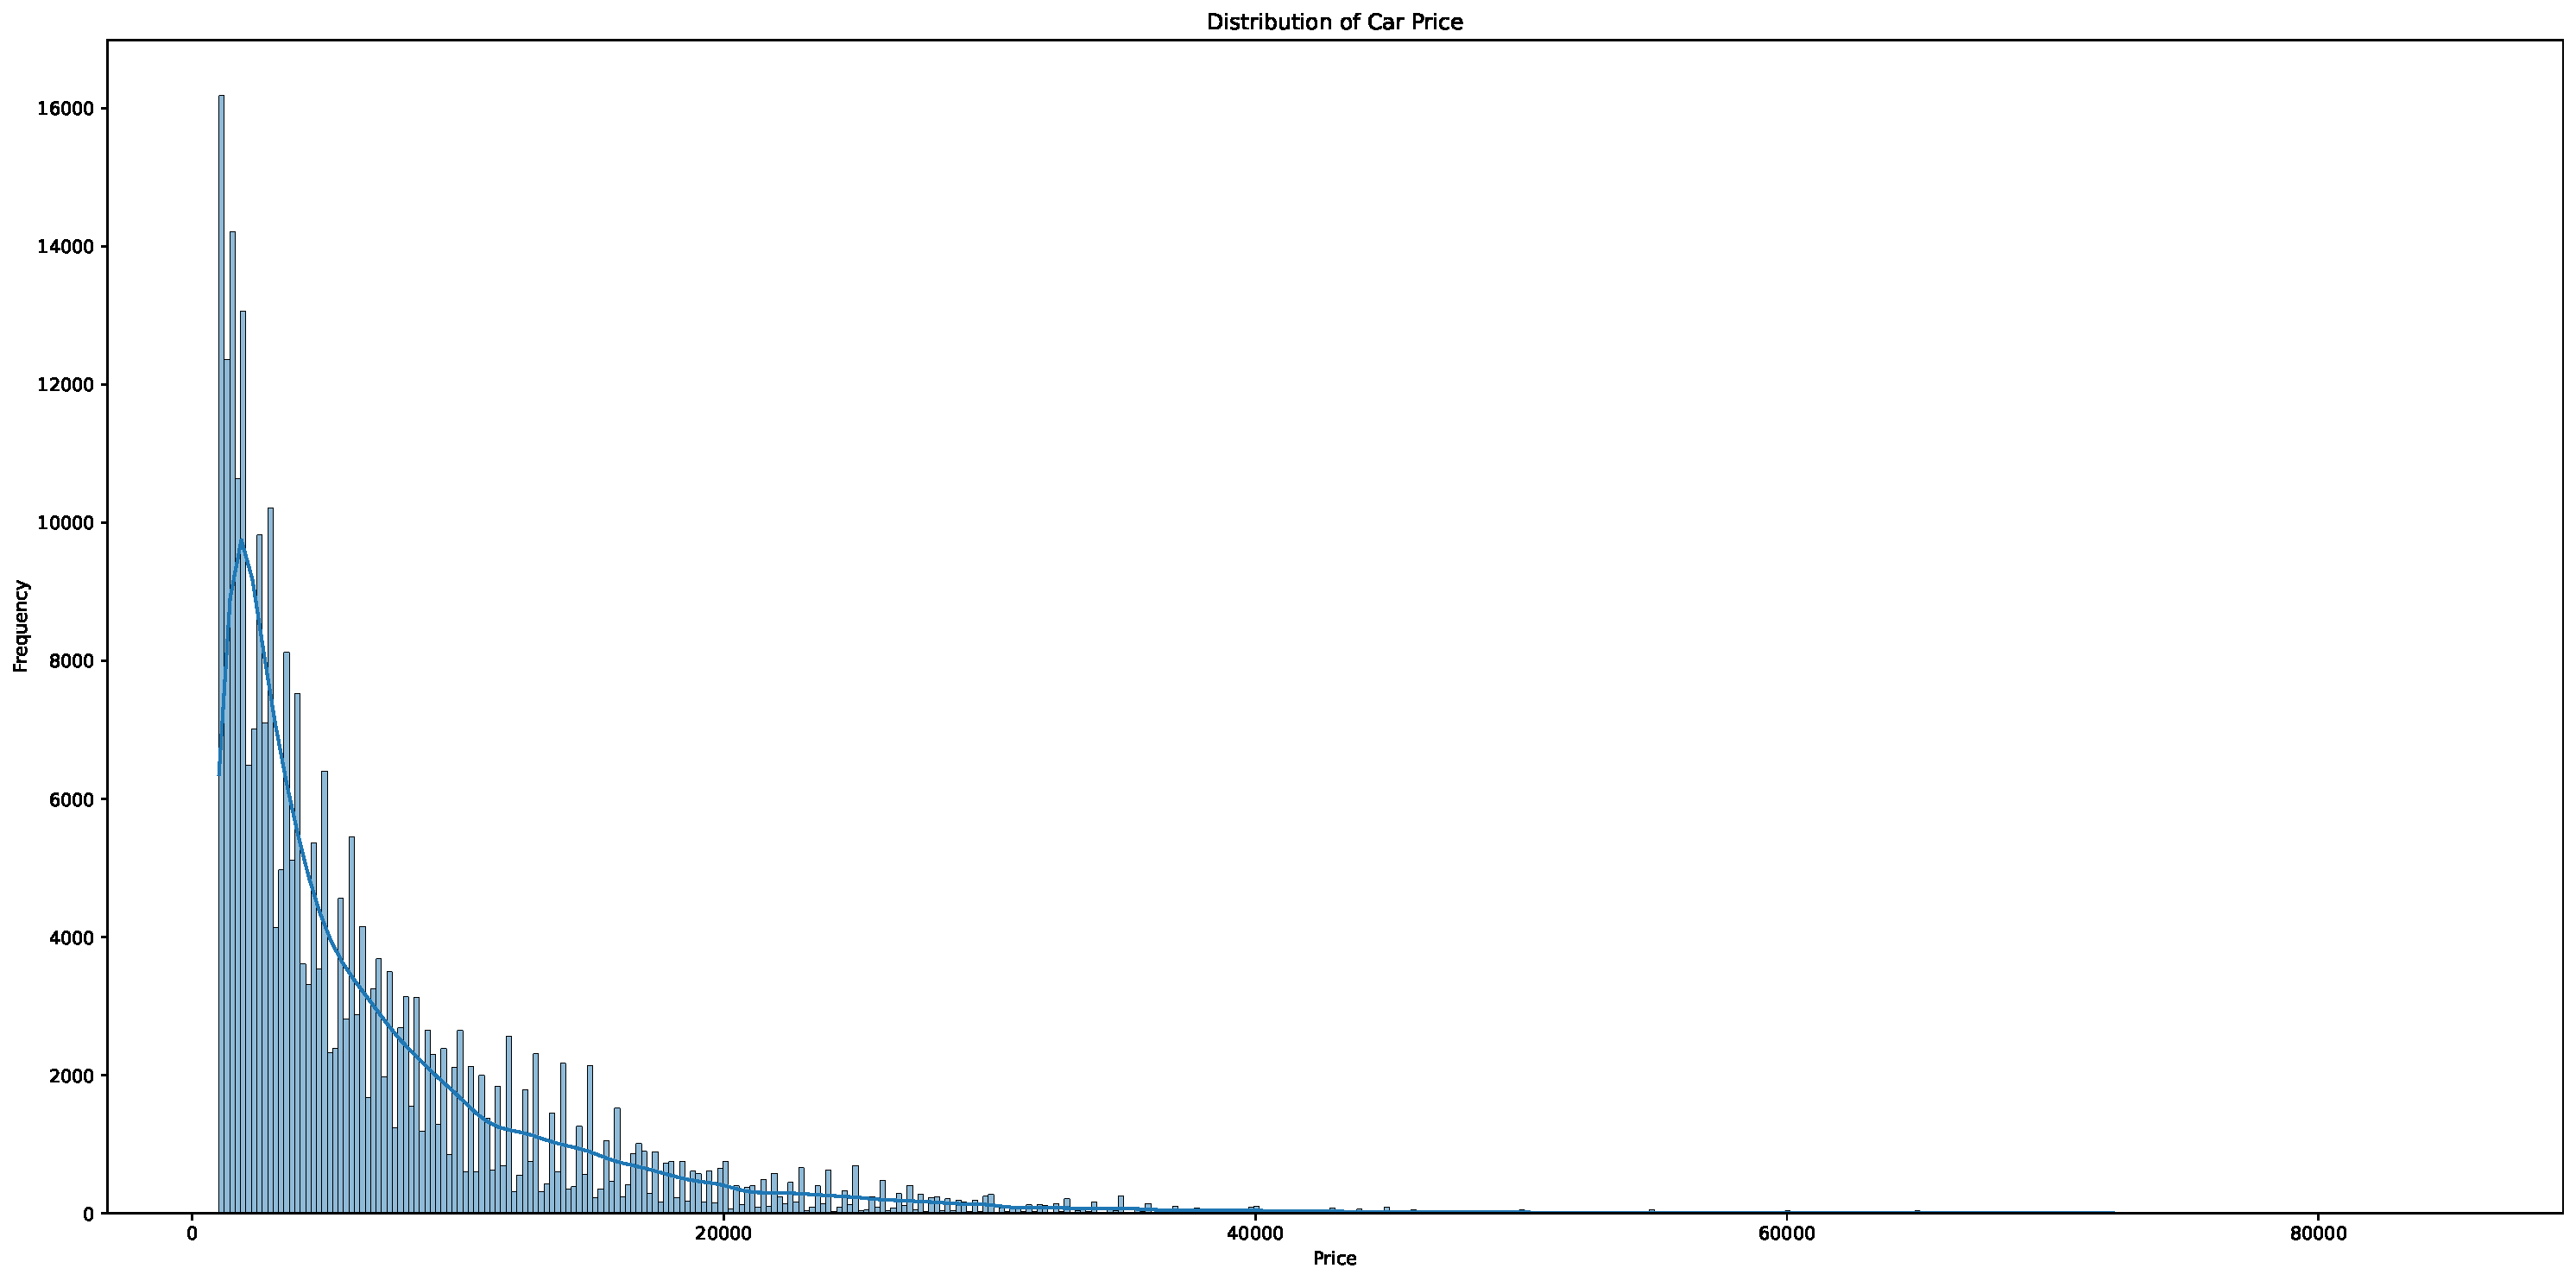
\includegraphics[width=\linewidth]{car_price_distribution.pdf}
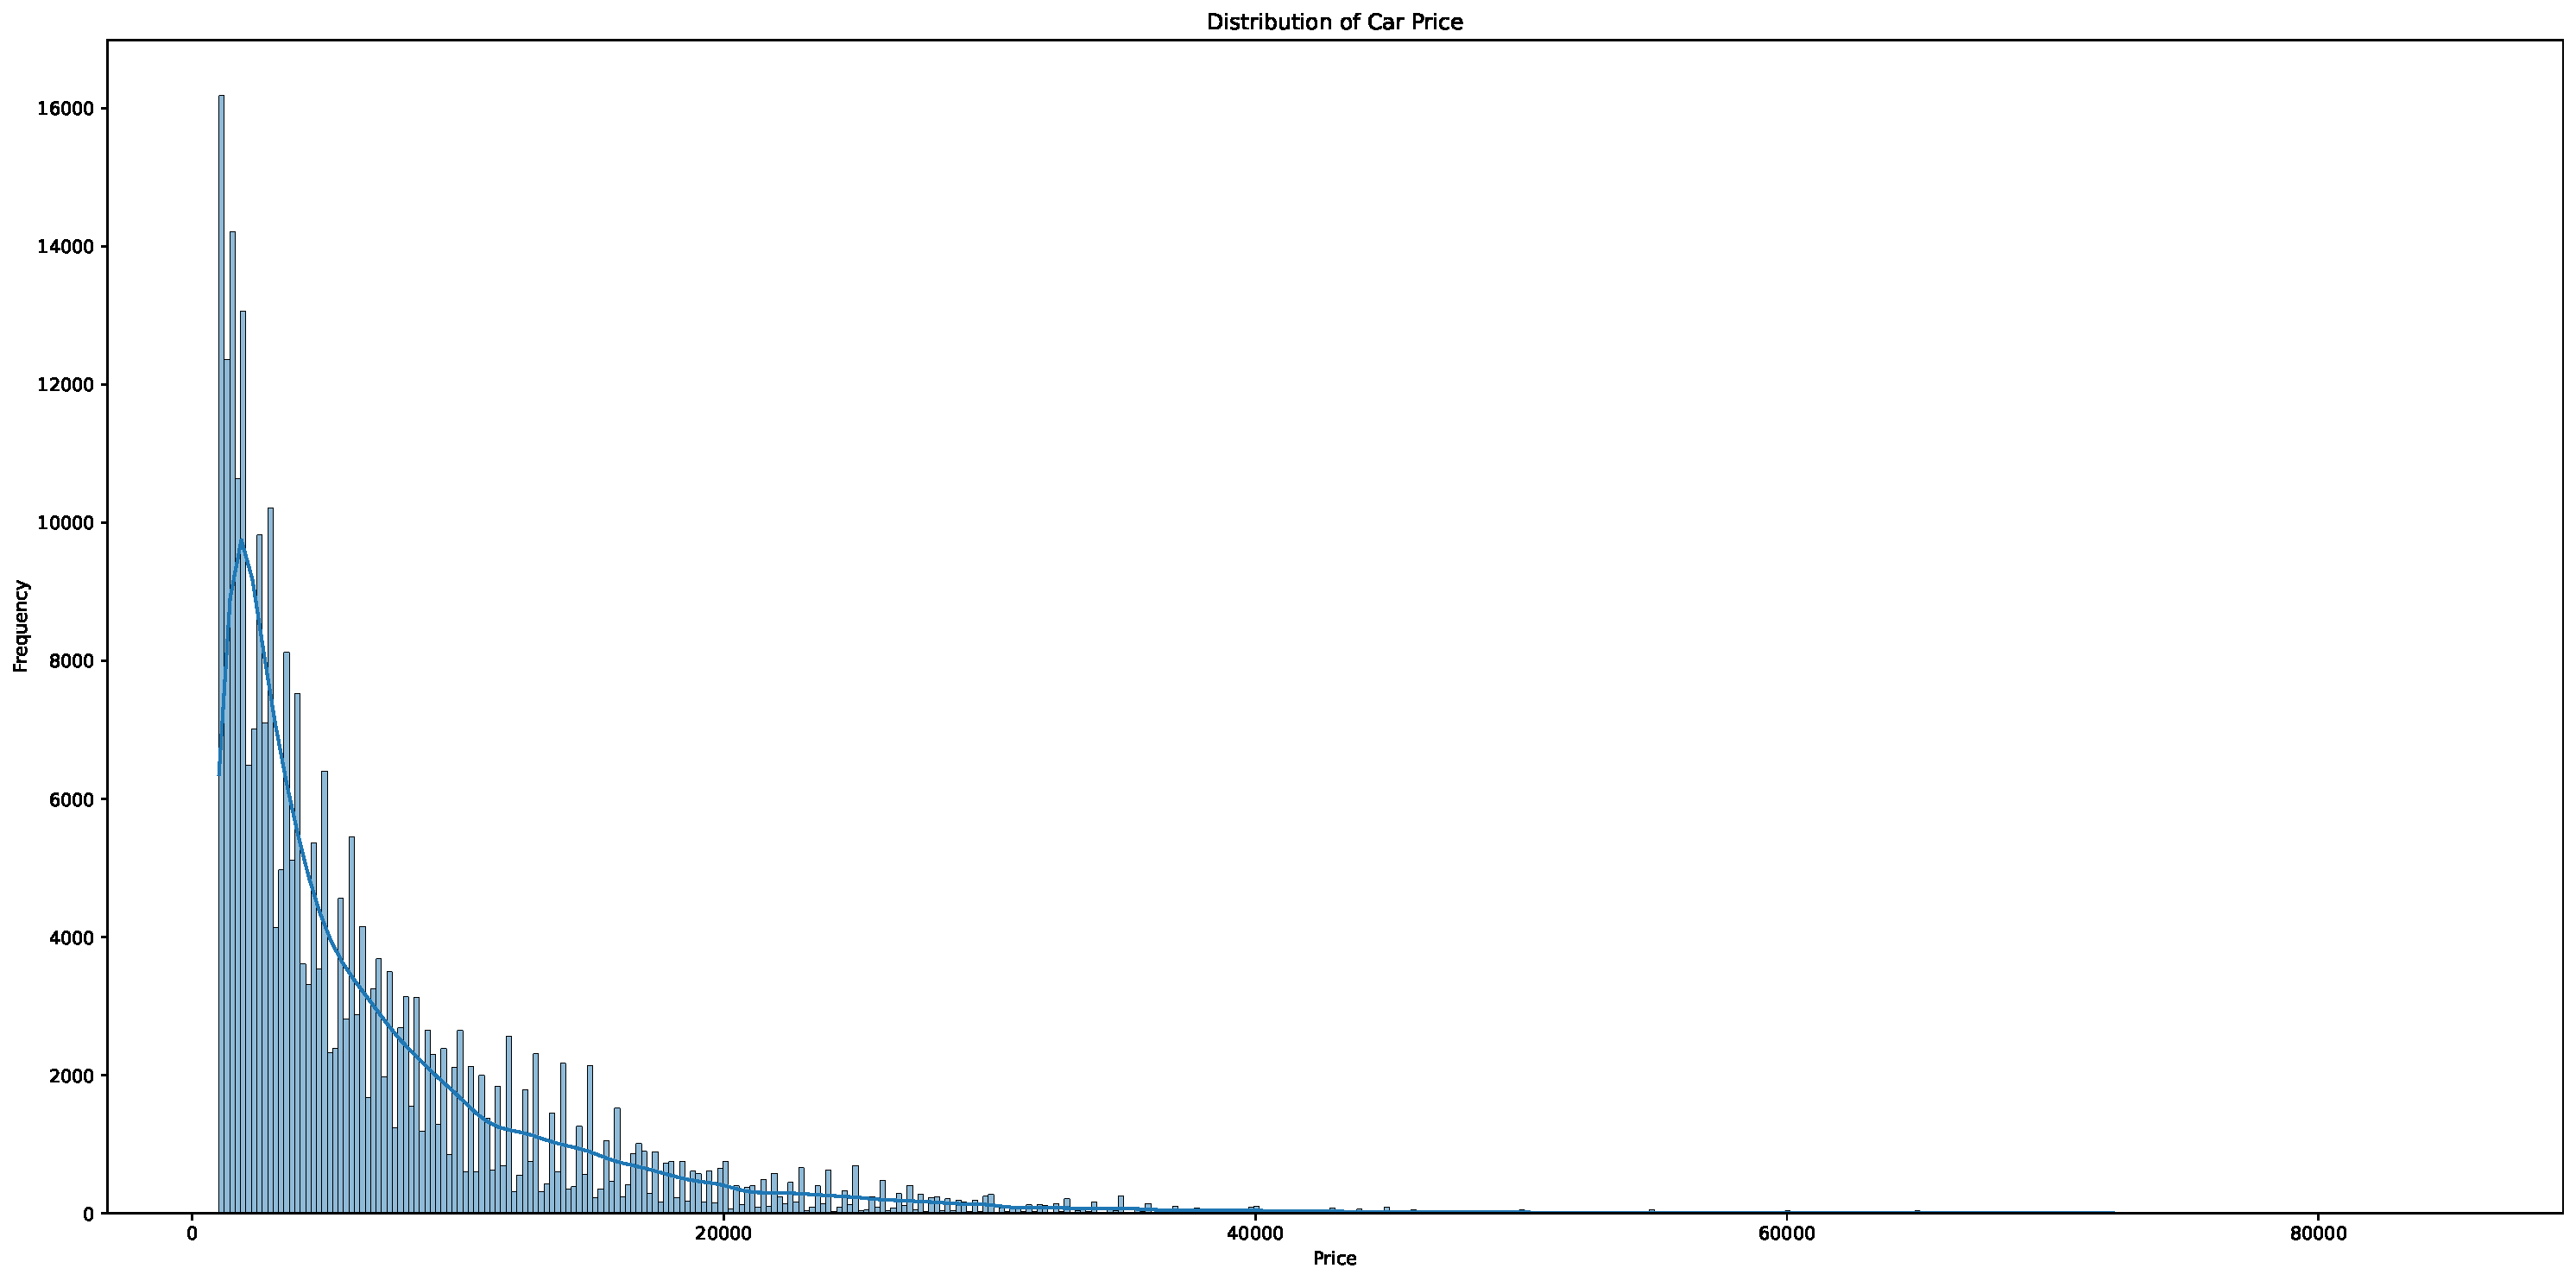
\includegraphics[scale=0.21]{car_price_distribution.pdf}
\end{frame}

\begin{frame}{Target Variable Analysis}
        \center
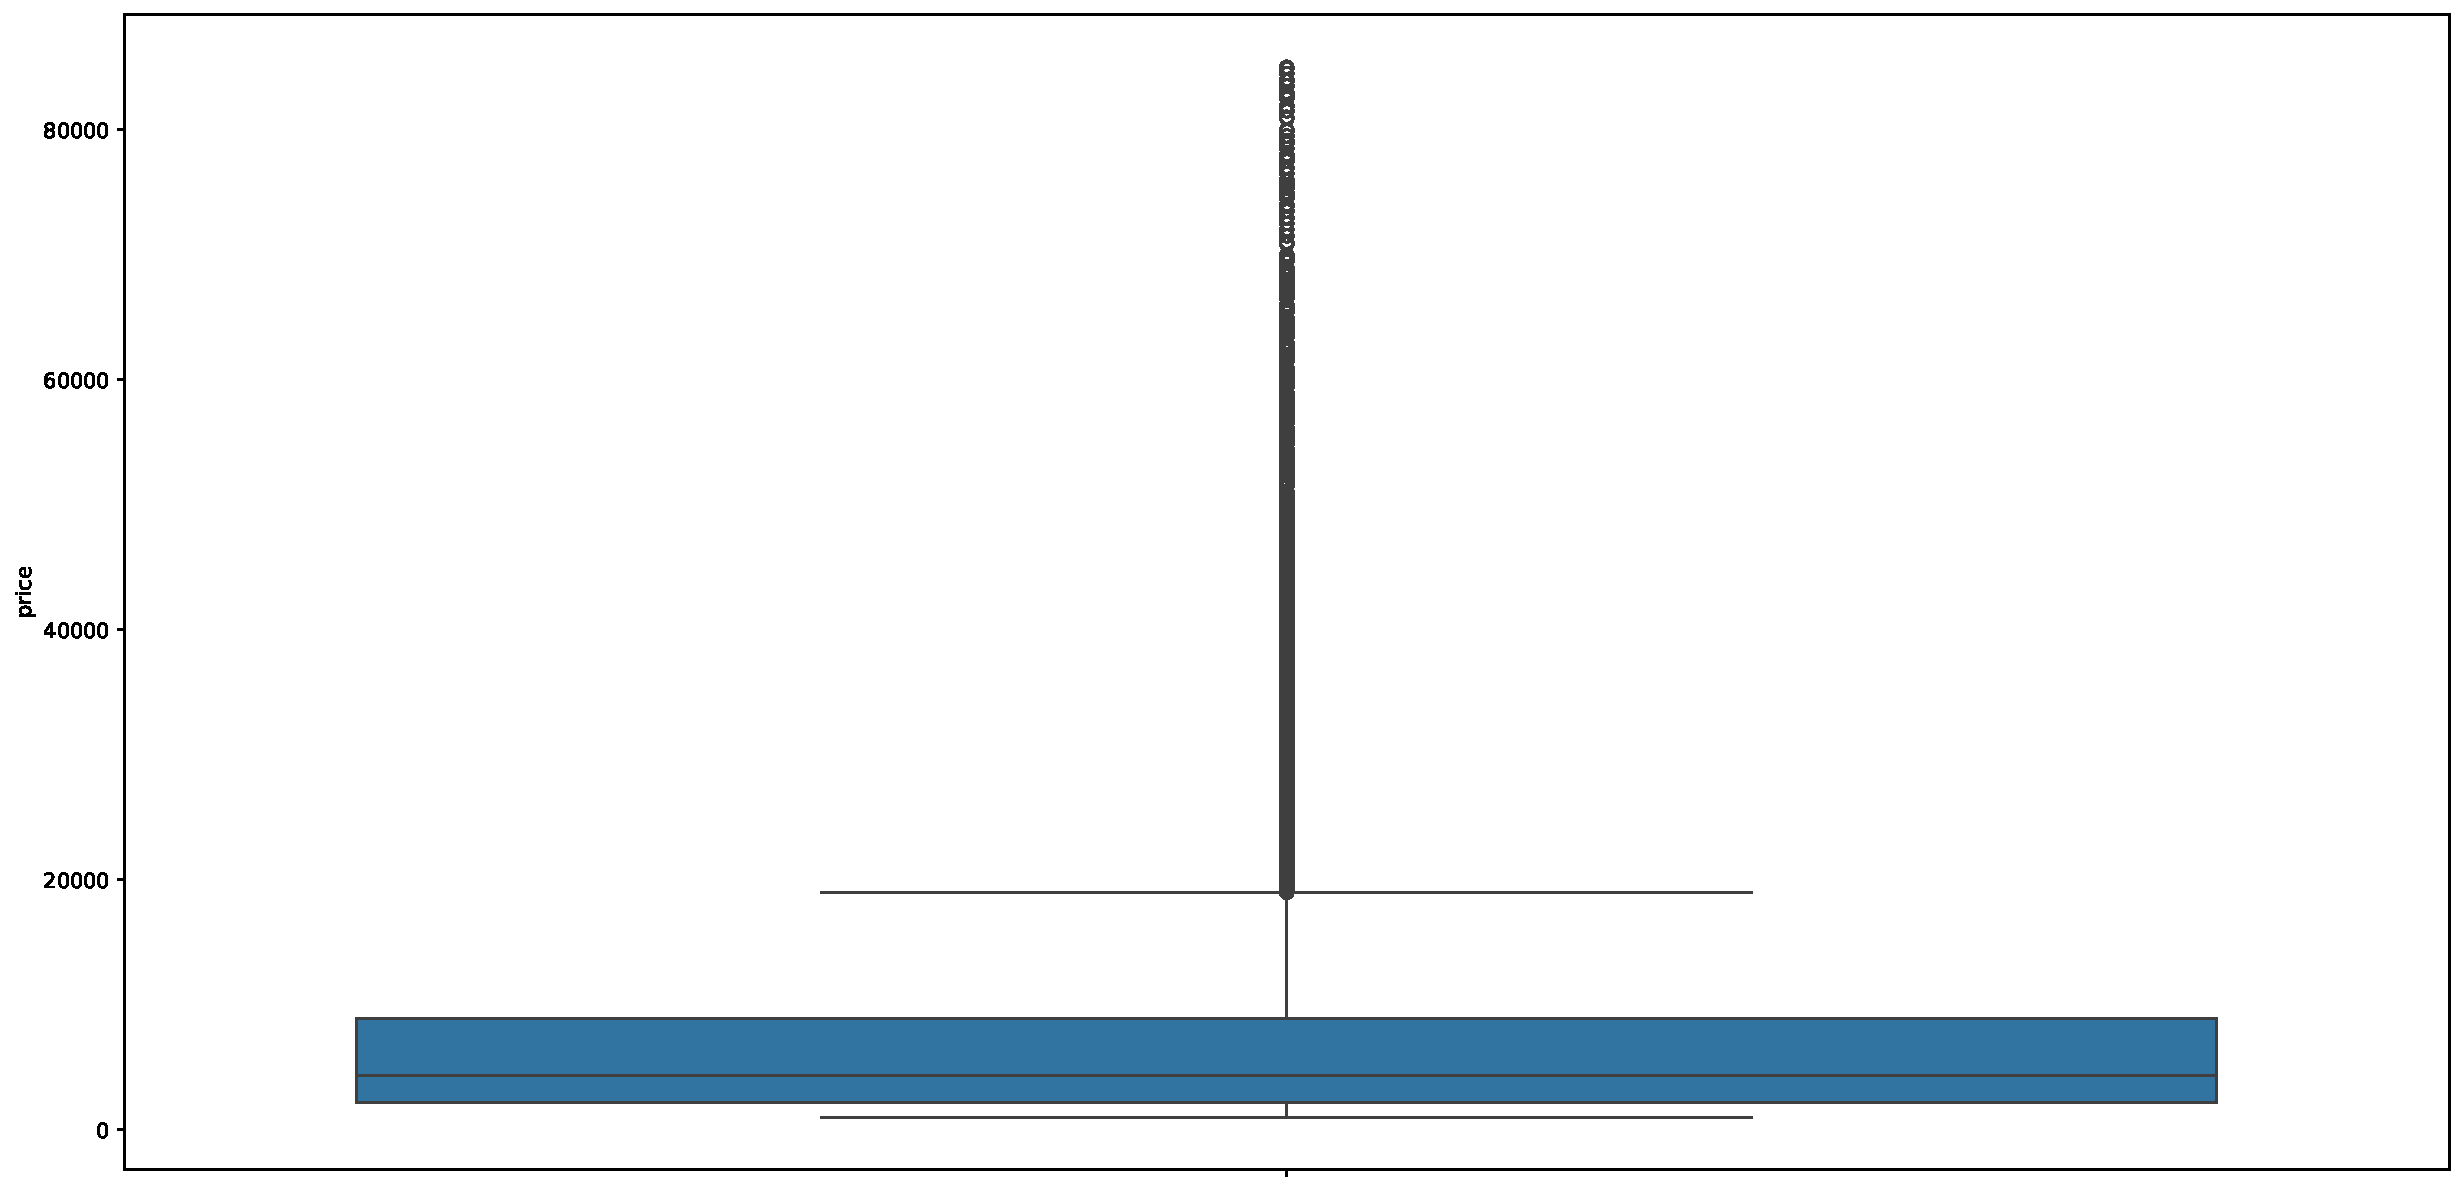
\includegraphics[scale=0.25]{car_price_boxplot.pdf}
\scriptsize 
Price boxplot
\end{frame}

\begin{frame}{Target Variable Analysis}
        \begin{itemize}
                \item The primary target is the car's selling \texttt{price}.
                \item \textbf{Distribution:} Price distribution is highly
                        right-skewed, with many extreme outliers.
                \item \textbf{Normality tests:} All tests (Anderson-Darling,
                        Kolmogorov-Smirnov, D’Agostino-Pearson, Jarque-Bera,
                        Lilliefors) indicate that \texttt{price} does
                        \textbf{not} follow a normal distribution.
                \item \textbf{Skewness:} 5.14 (very high, confirms extreme
                        right skew).
                \item \textbf{Implications:}
                        \begin{itemize}
                                \item Model will perform best on low/average
                                        prices, but may struggle with
                                        high-price cars due to data imbalance.
                                \item Considered unskewing techniques such as
                                        Box-Cox and Yeo-Johnson.
                        \end{itemize}
        \end{itemize}
\end{frame}


\begin{frame}{Categorical Features Analysis}
        \center
        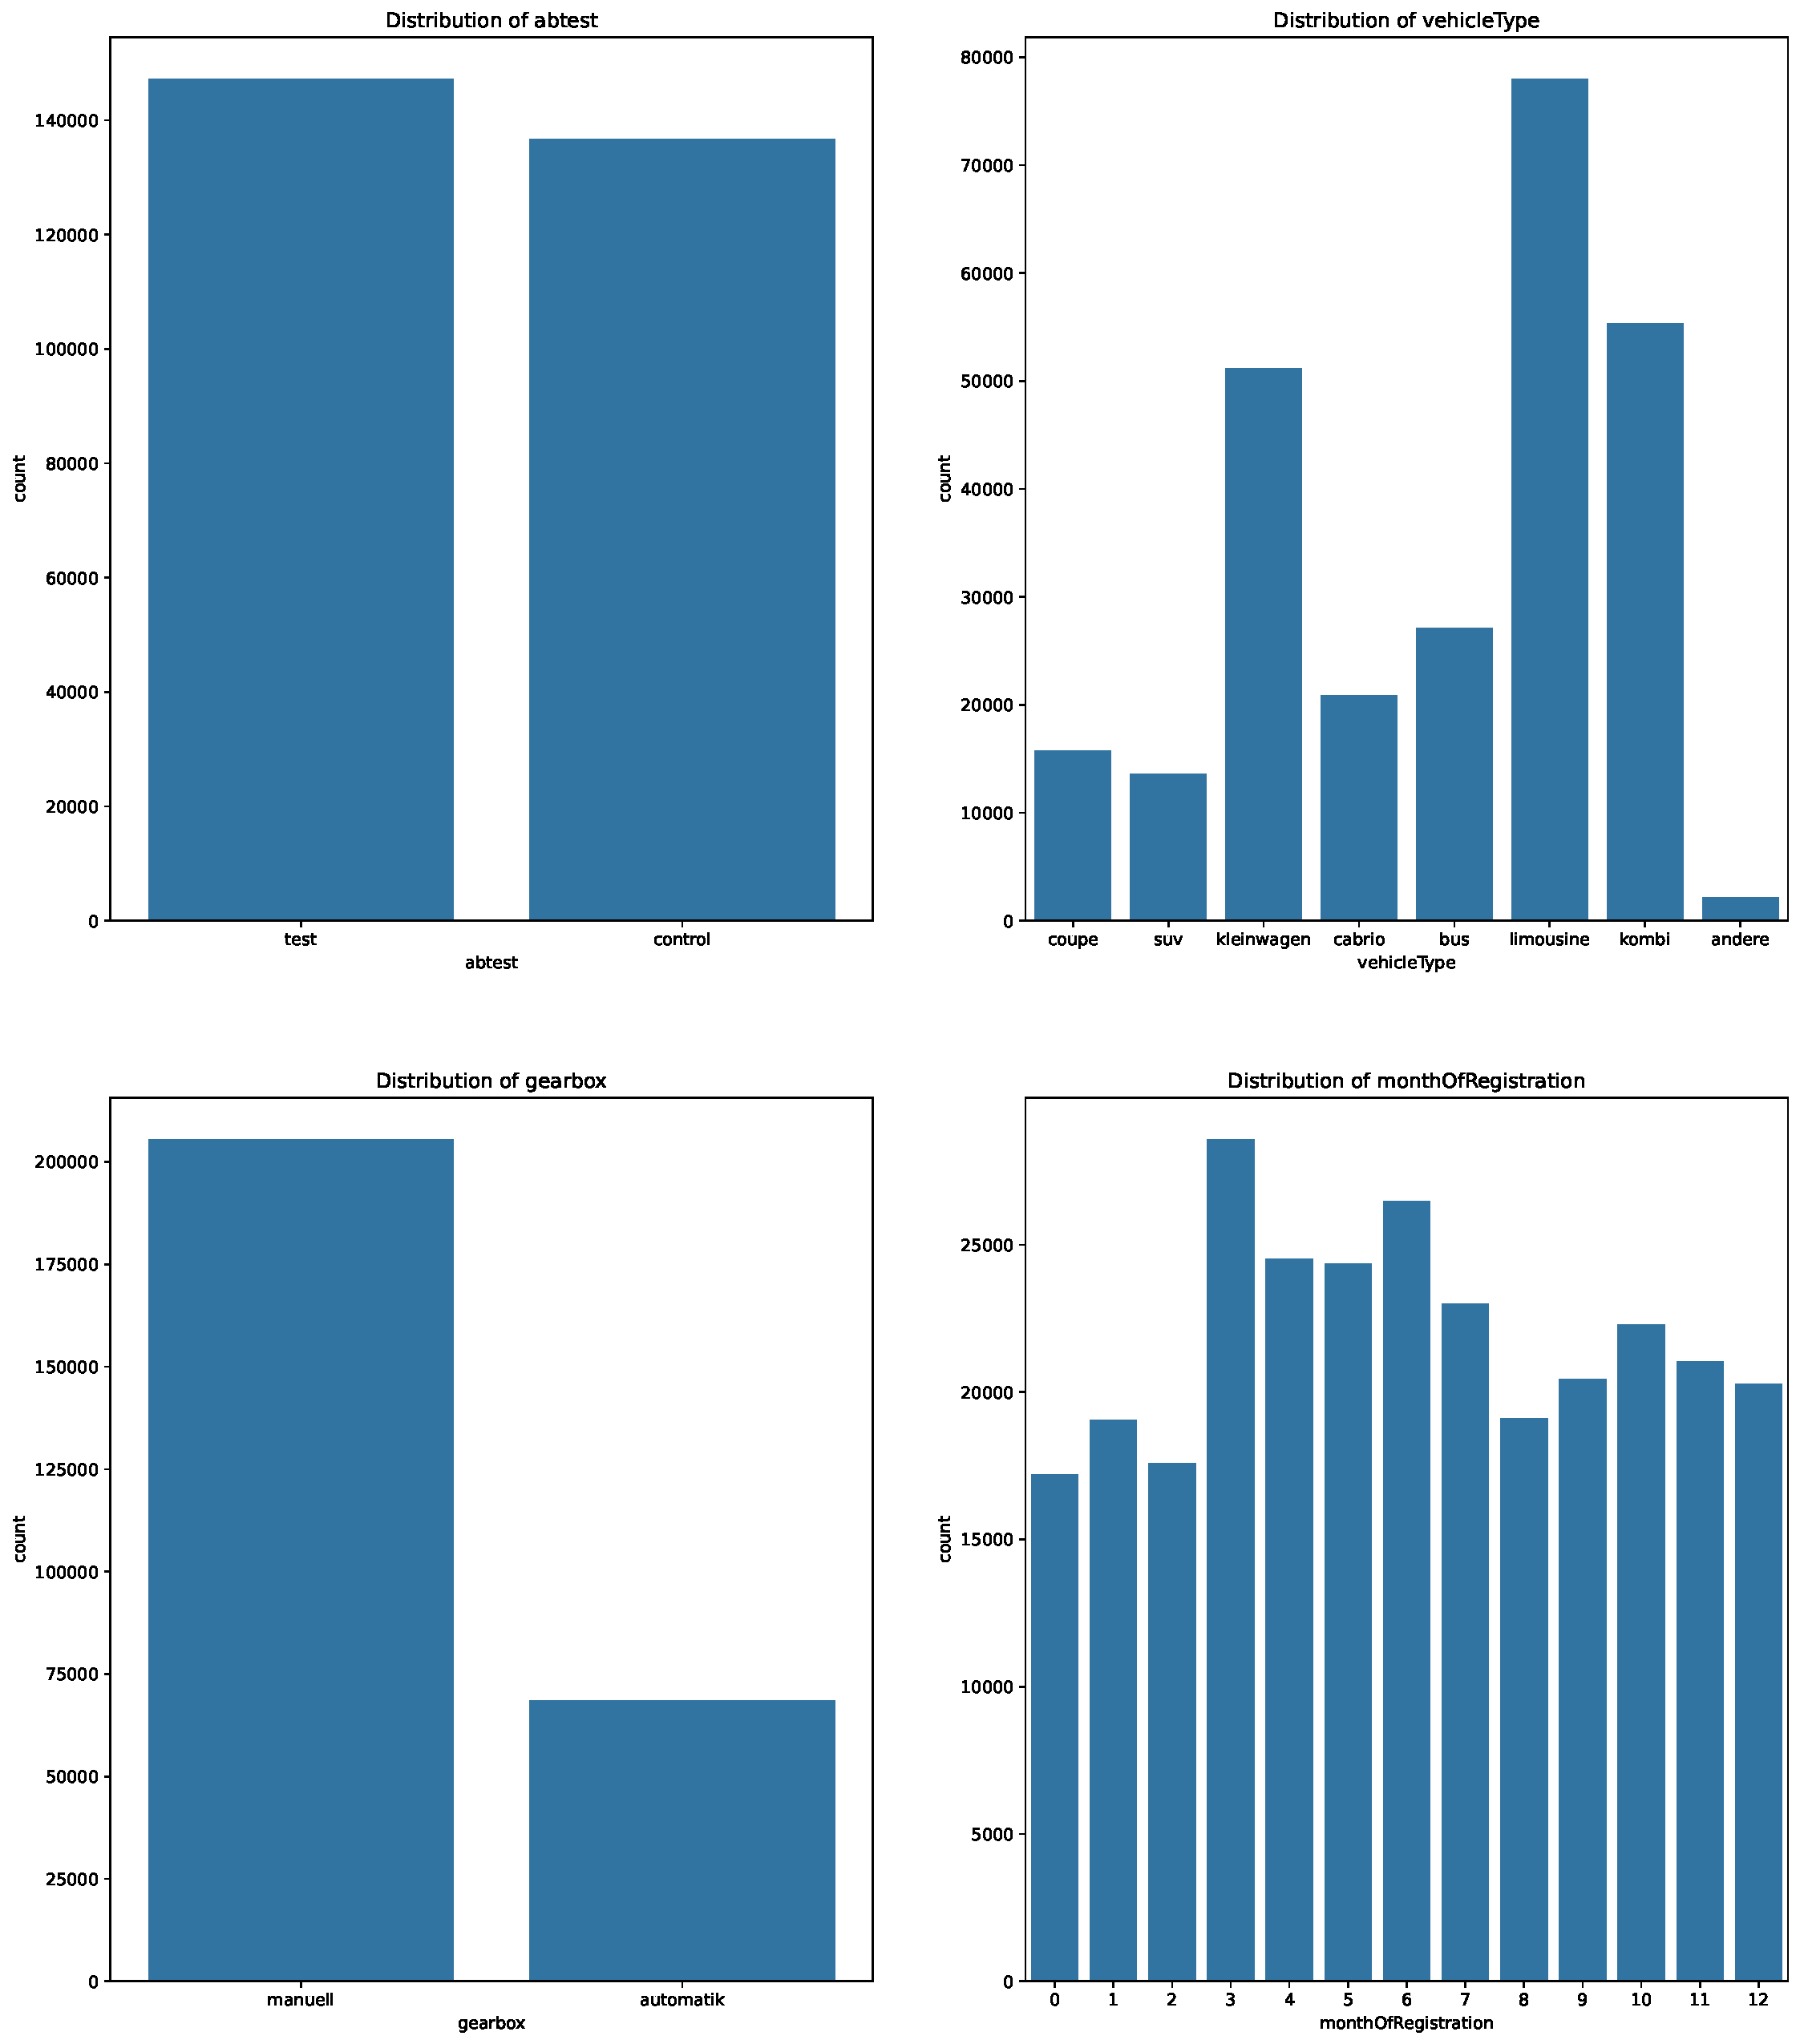
\includegraphics[scale=0.2]{cat_features_distribution1.pdf}
\end{frame}

\begin{frame}{Categorical Features Analysis}
        \center
        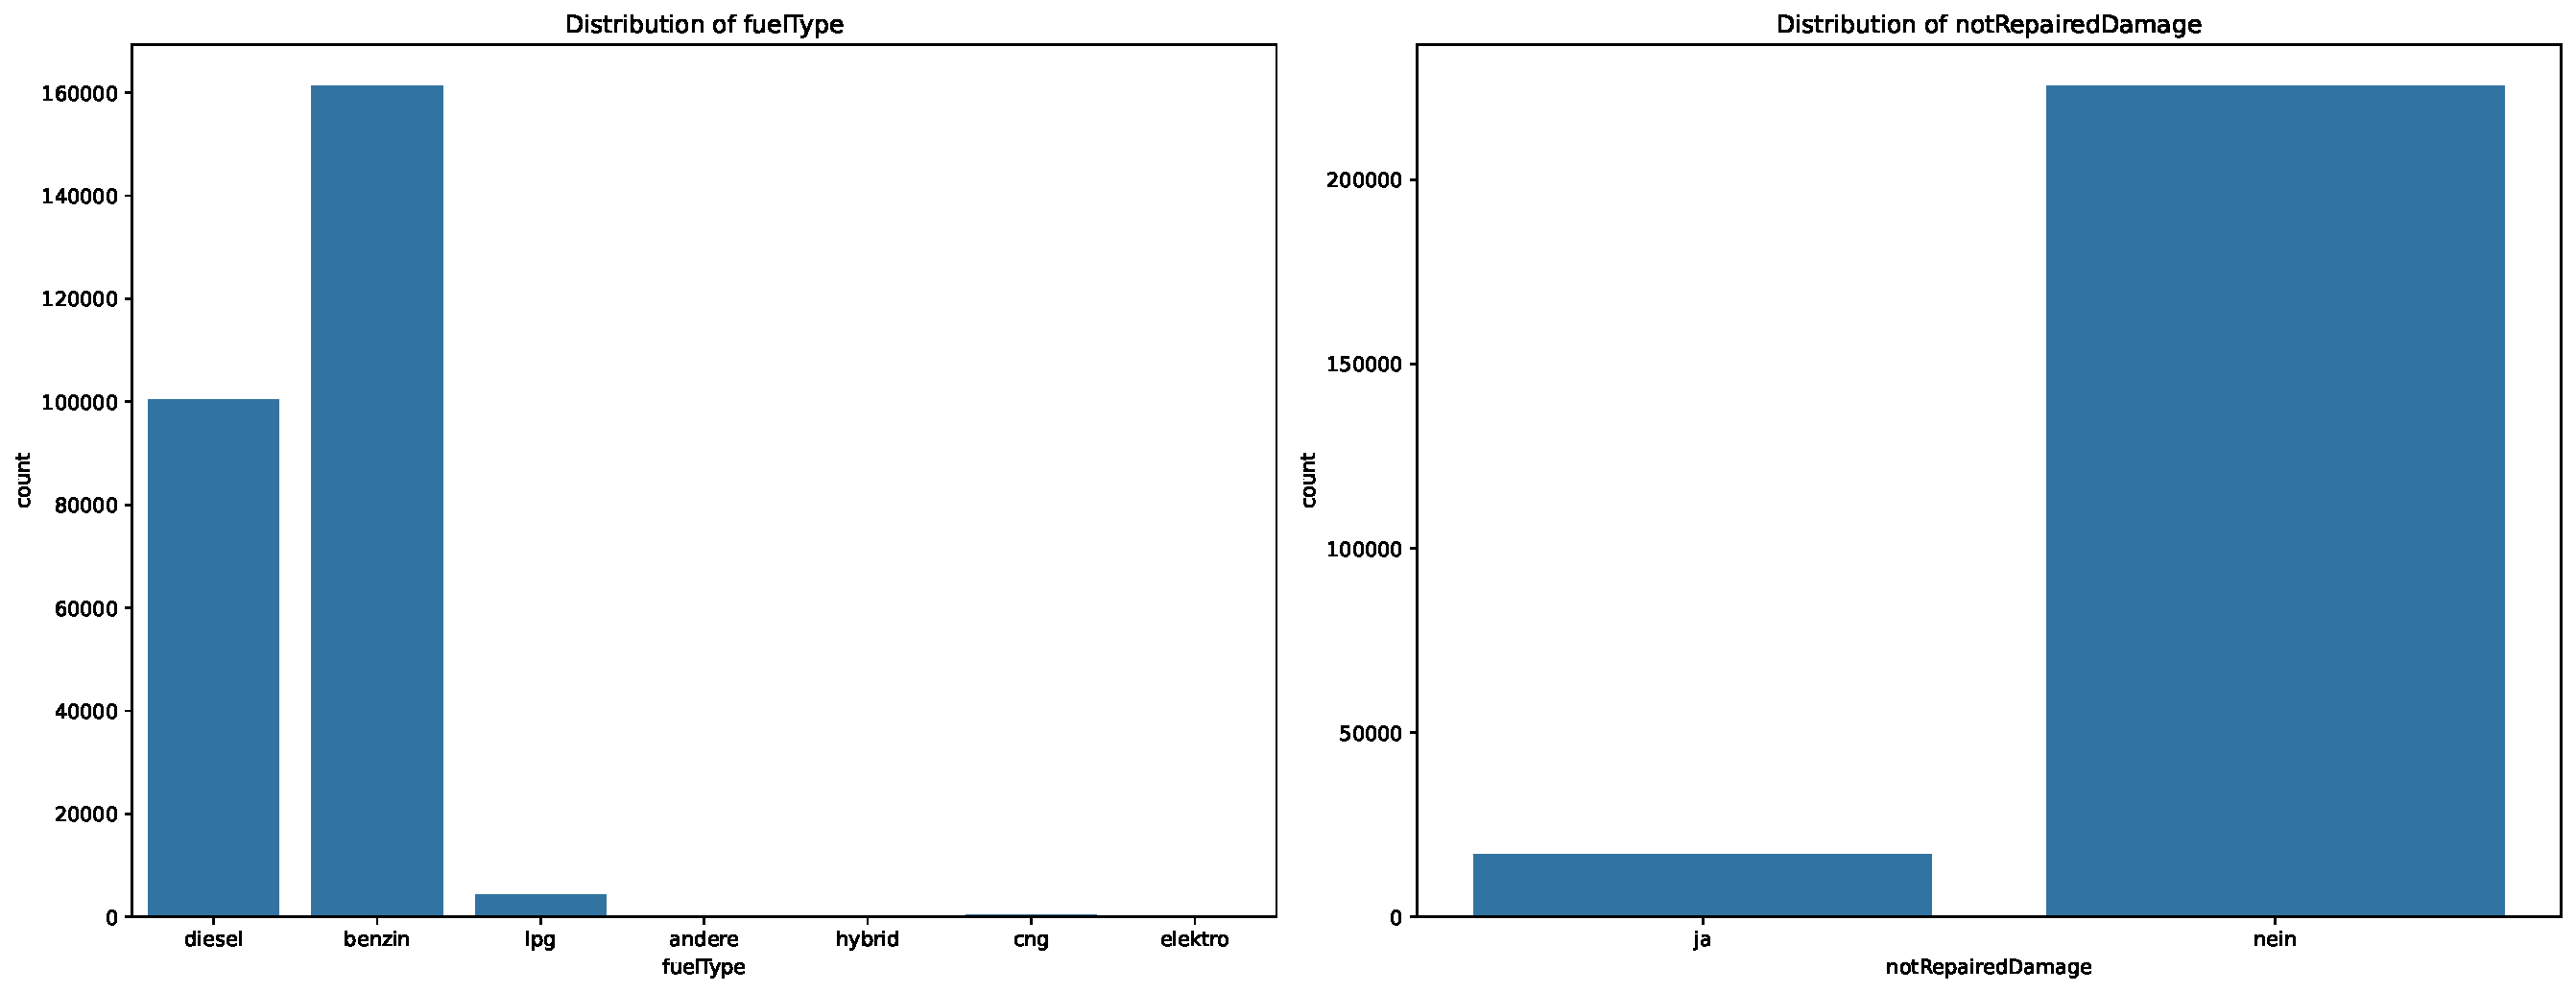
\includegraphics[scale=0.22]{cat_features_distribution2.pdf}
        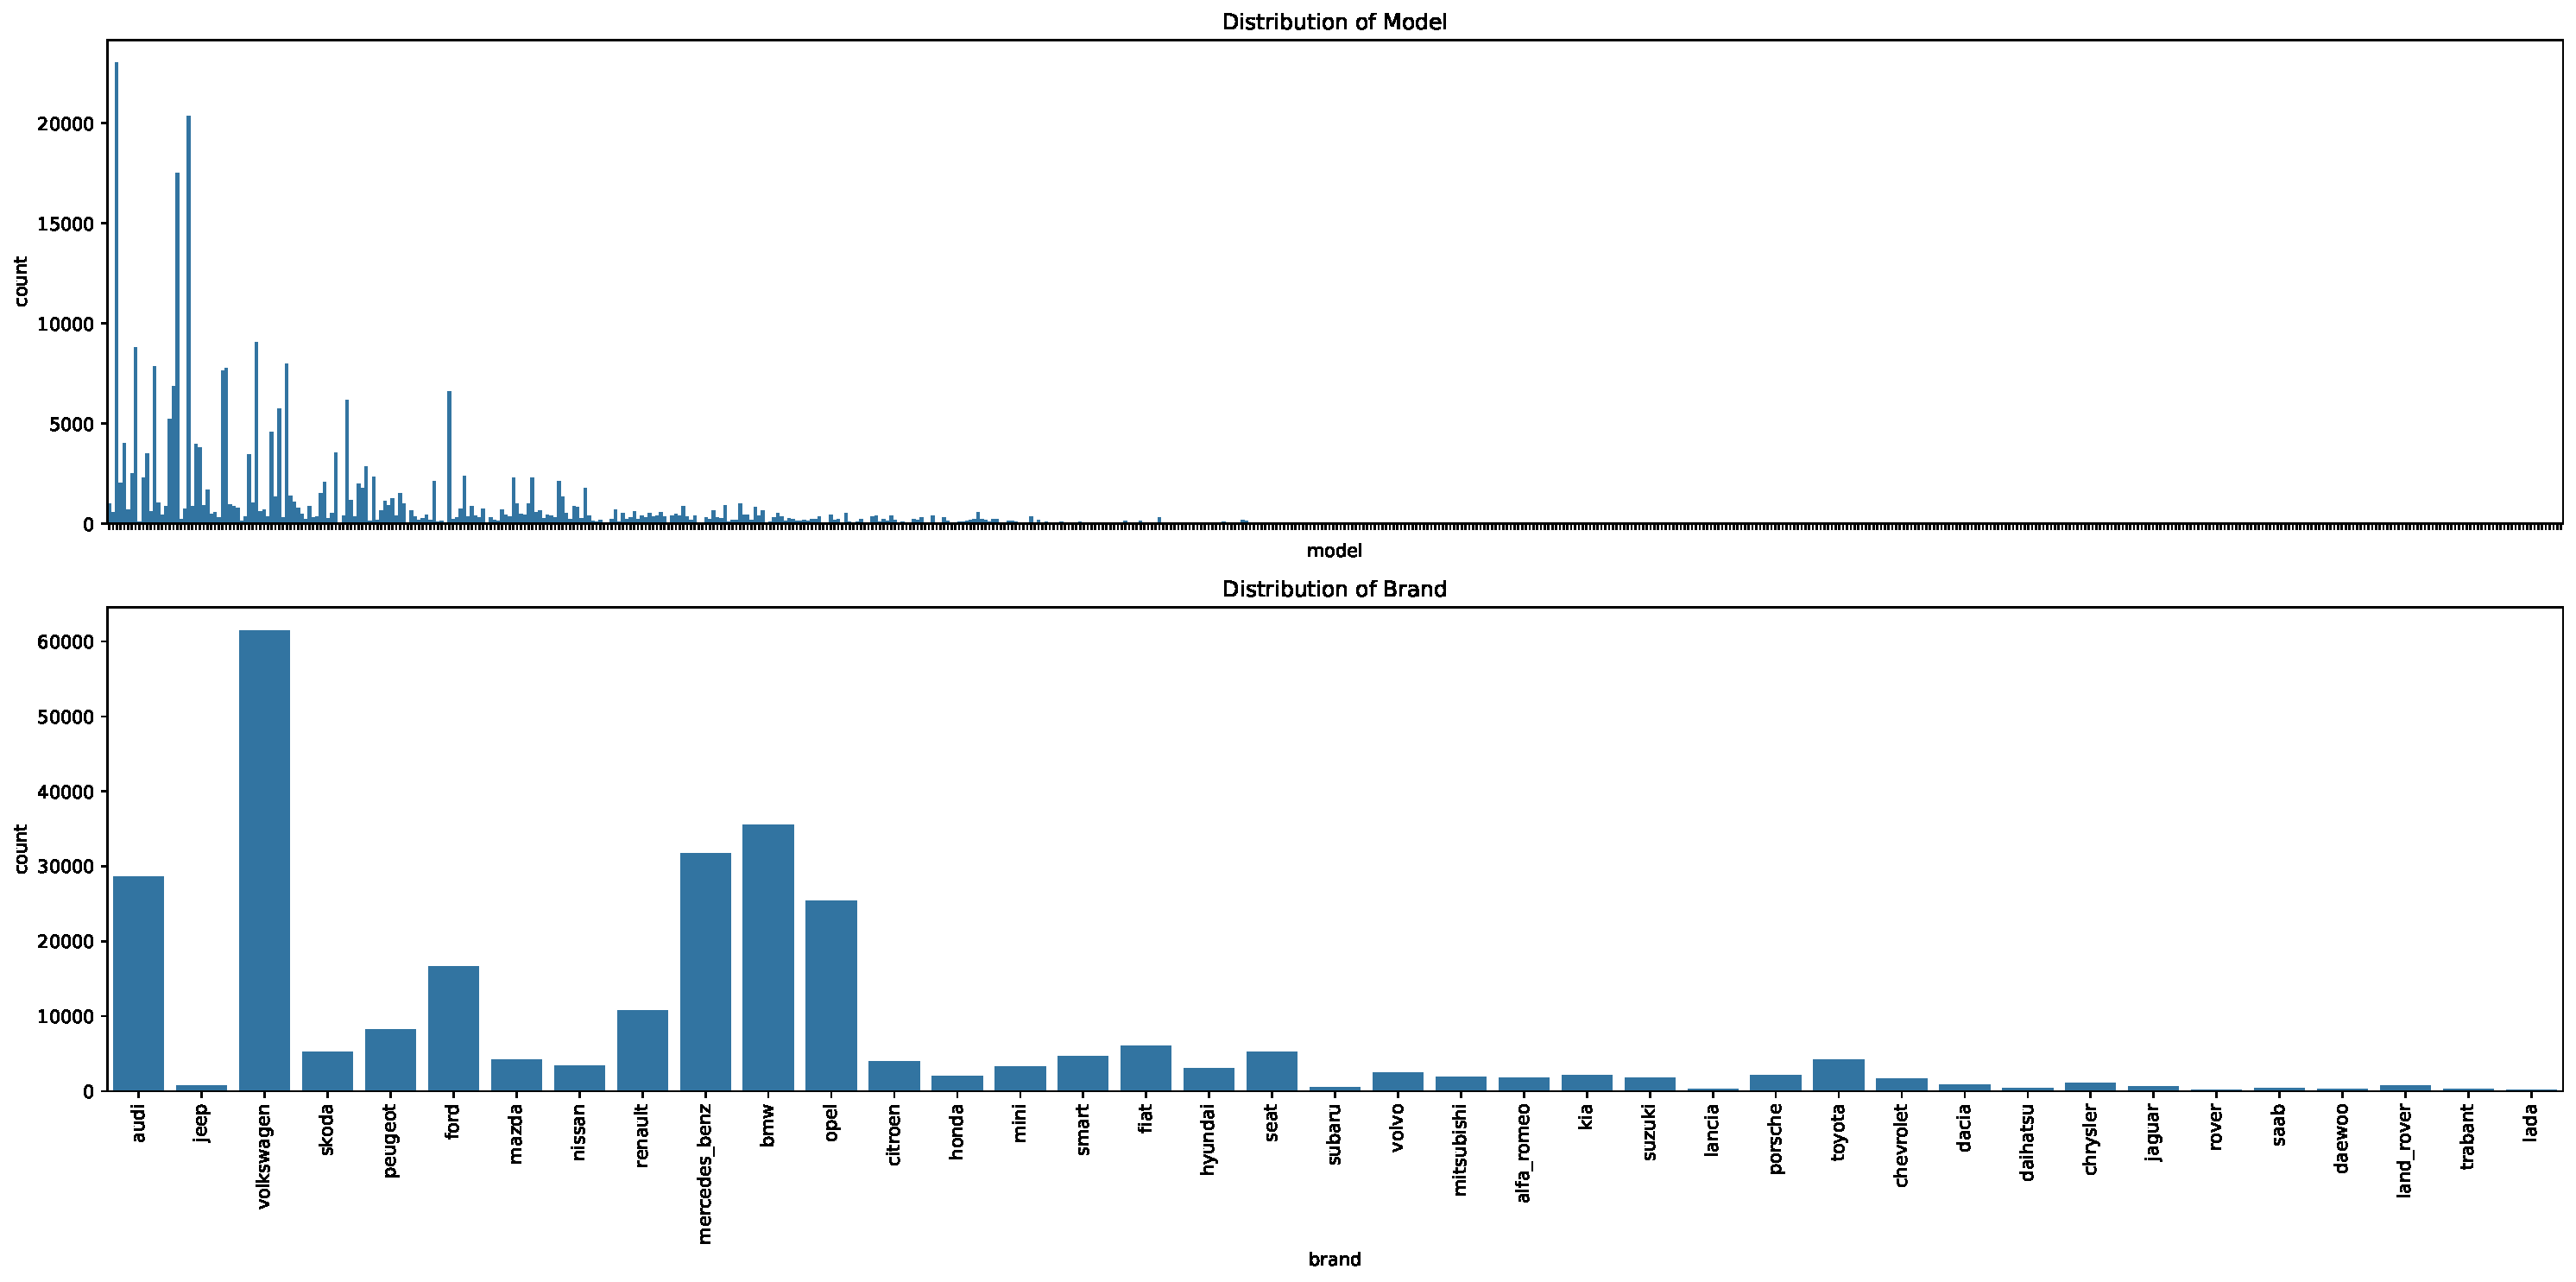
\includegraphics[scale=0.2]{model_brand_distribution.pdf}
\end{frame}

\begin{frame}{Categorical Features Analysis}
        \center
        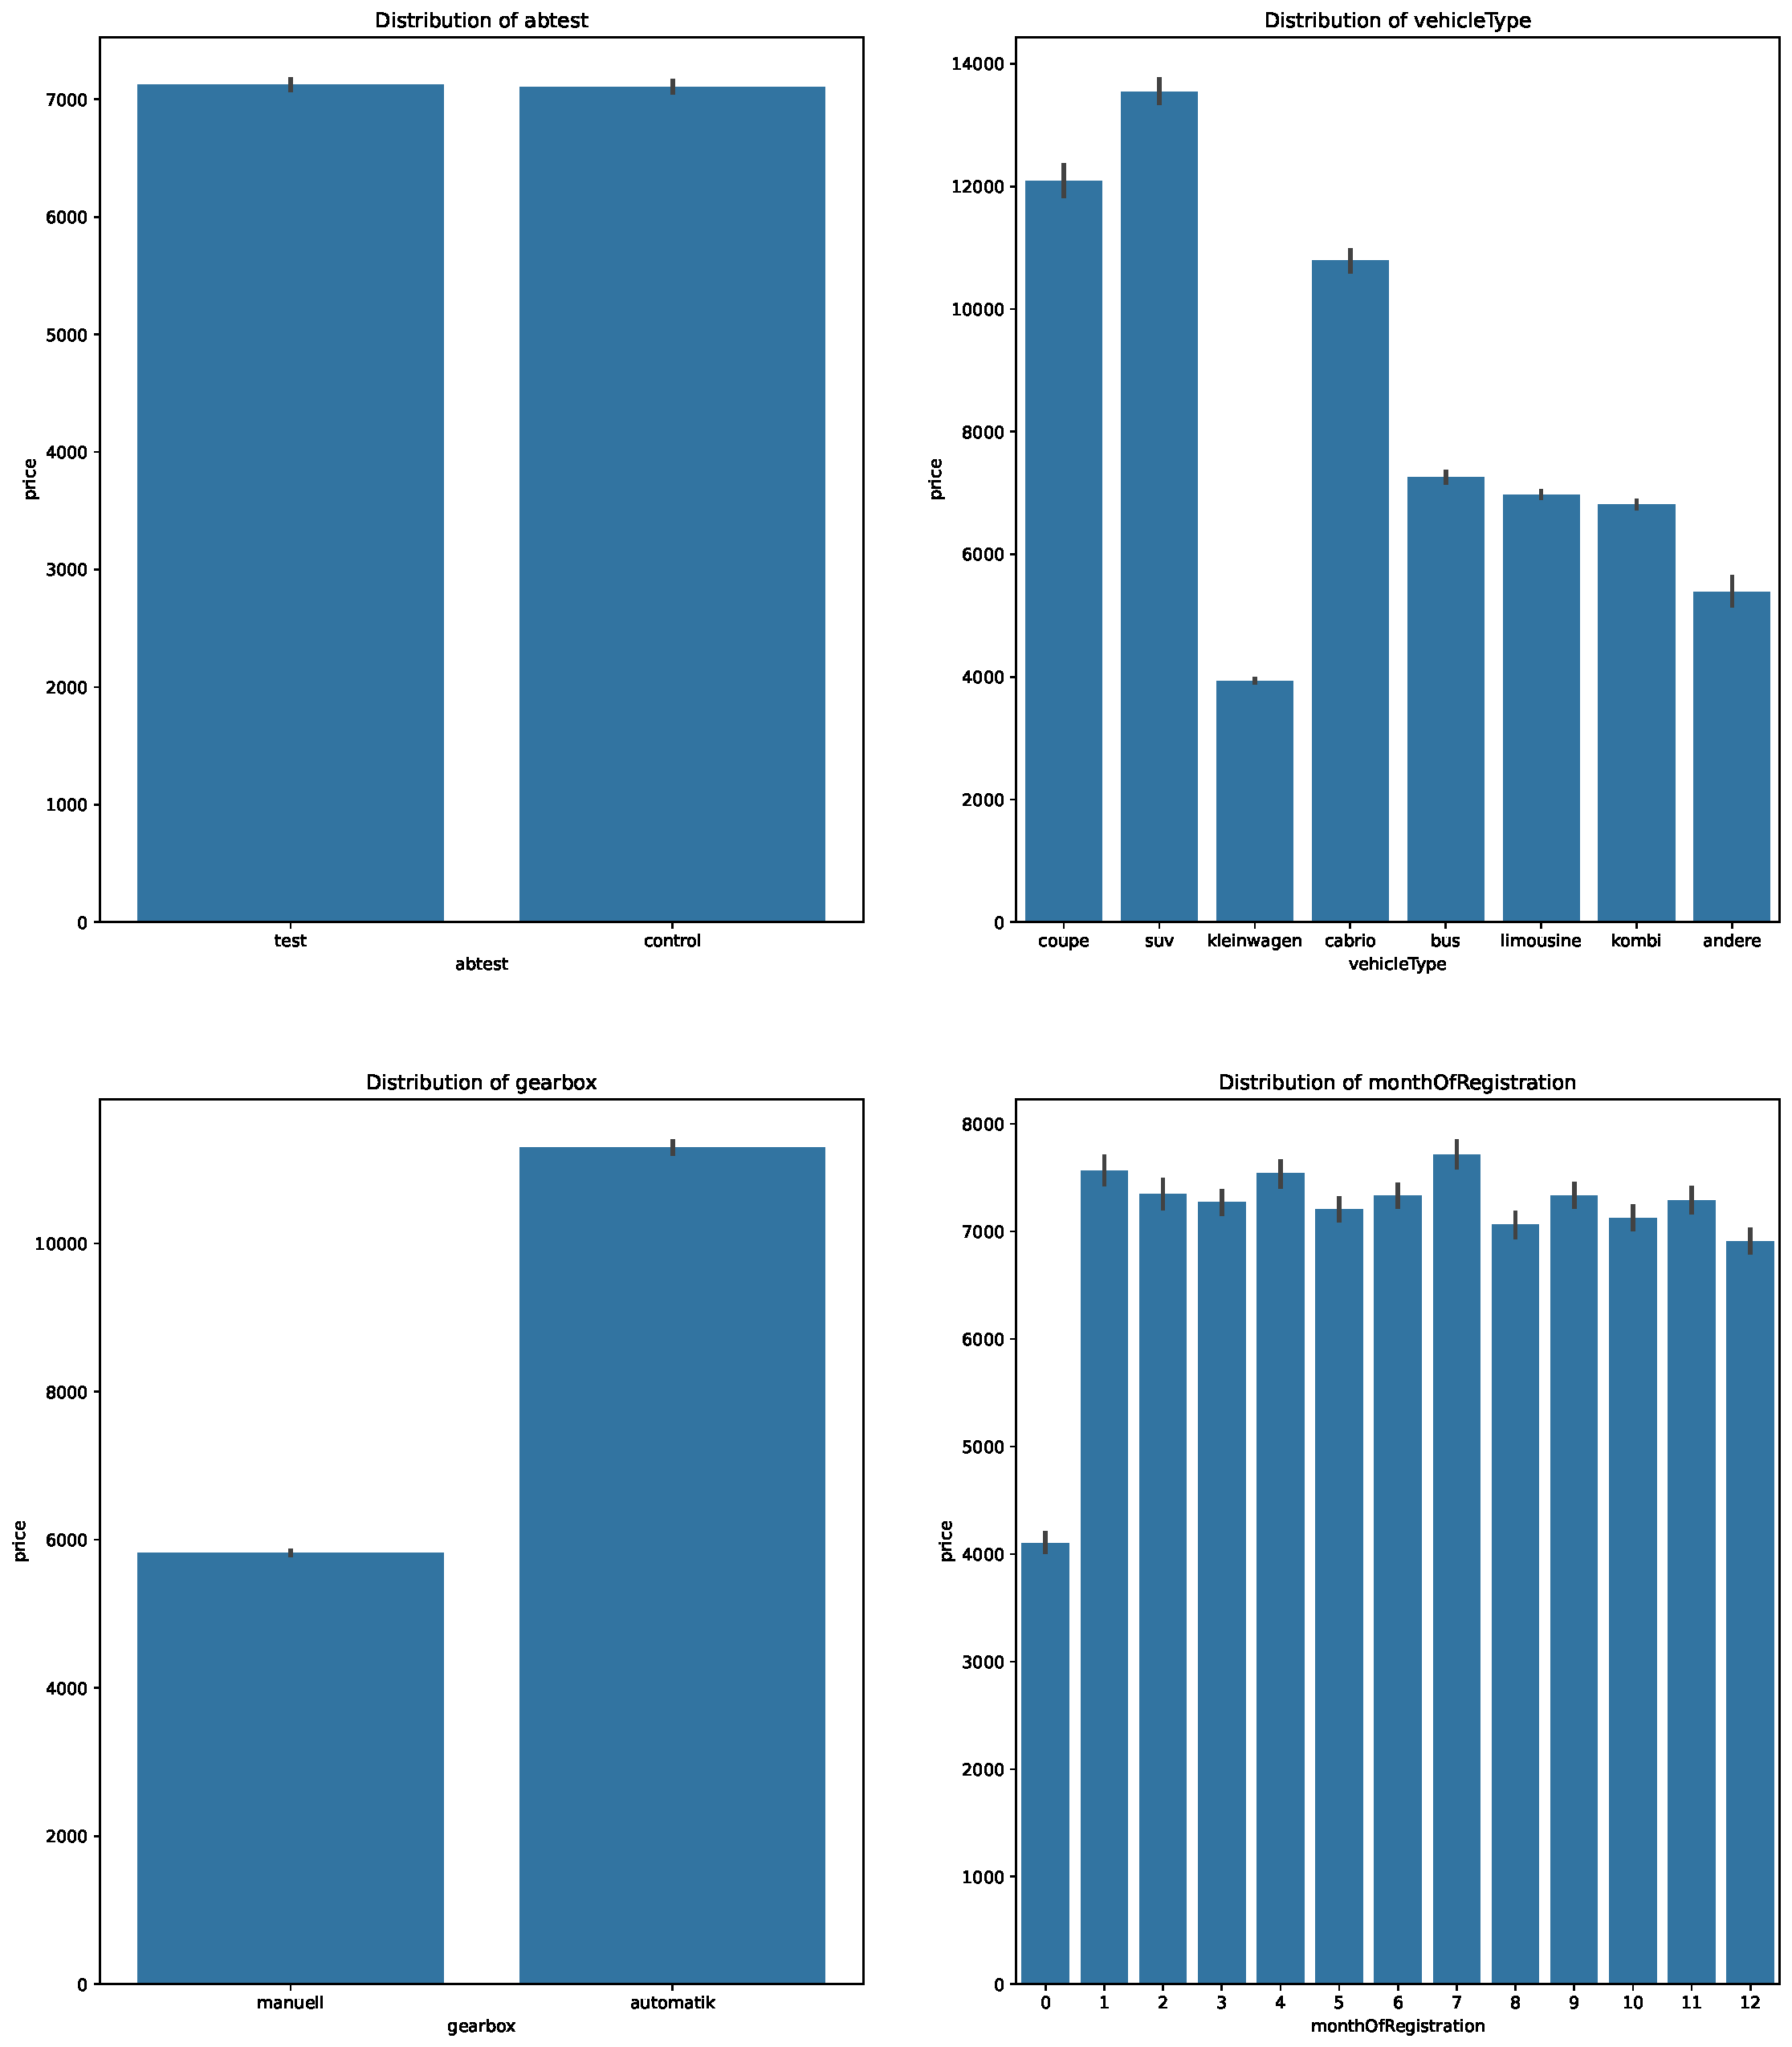
\includegraphics[scale=0.2]{cat_features_barplot1.pdf}
\end{frame}

\begin{frame}{Categorical Features Analysis}
        \center
        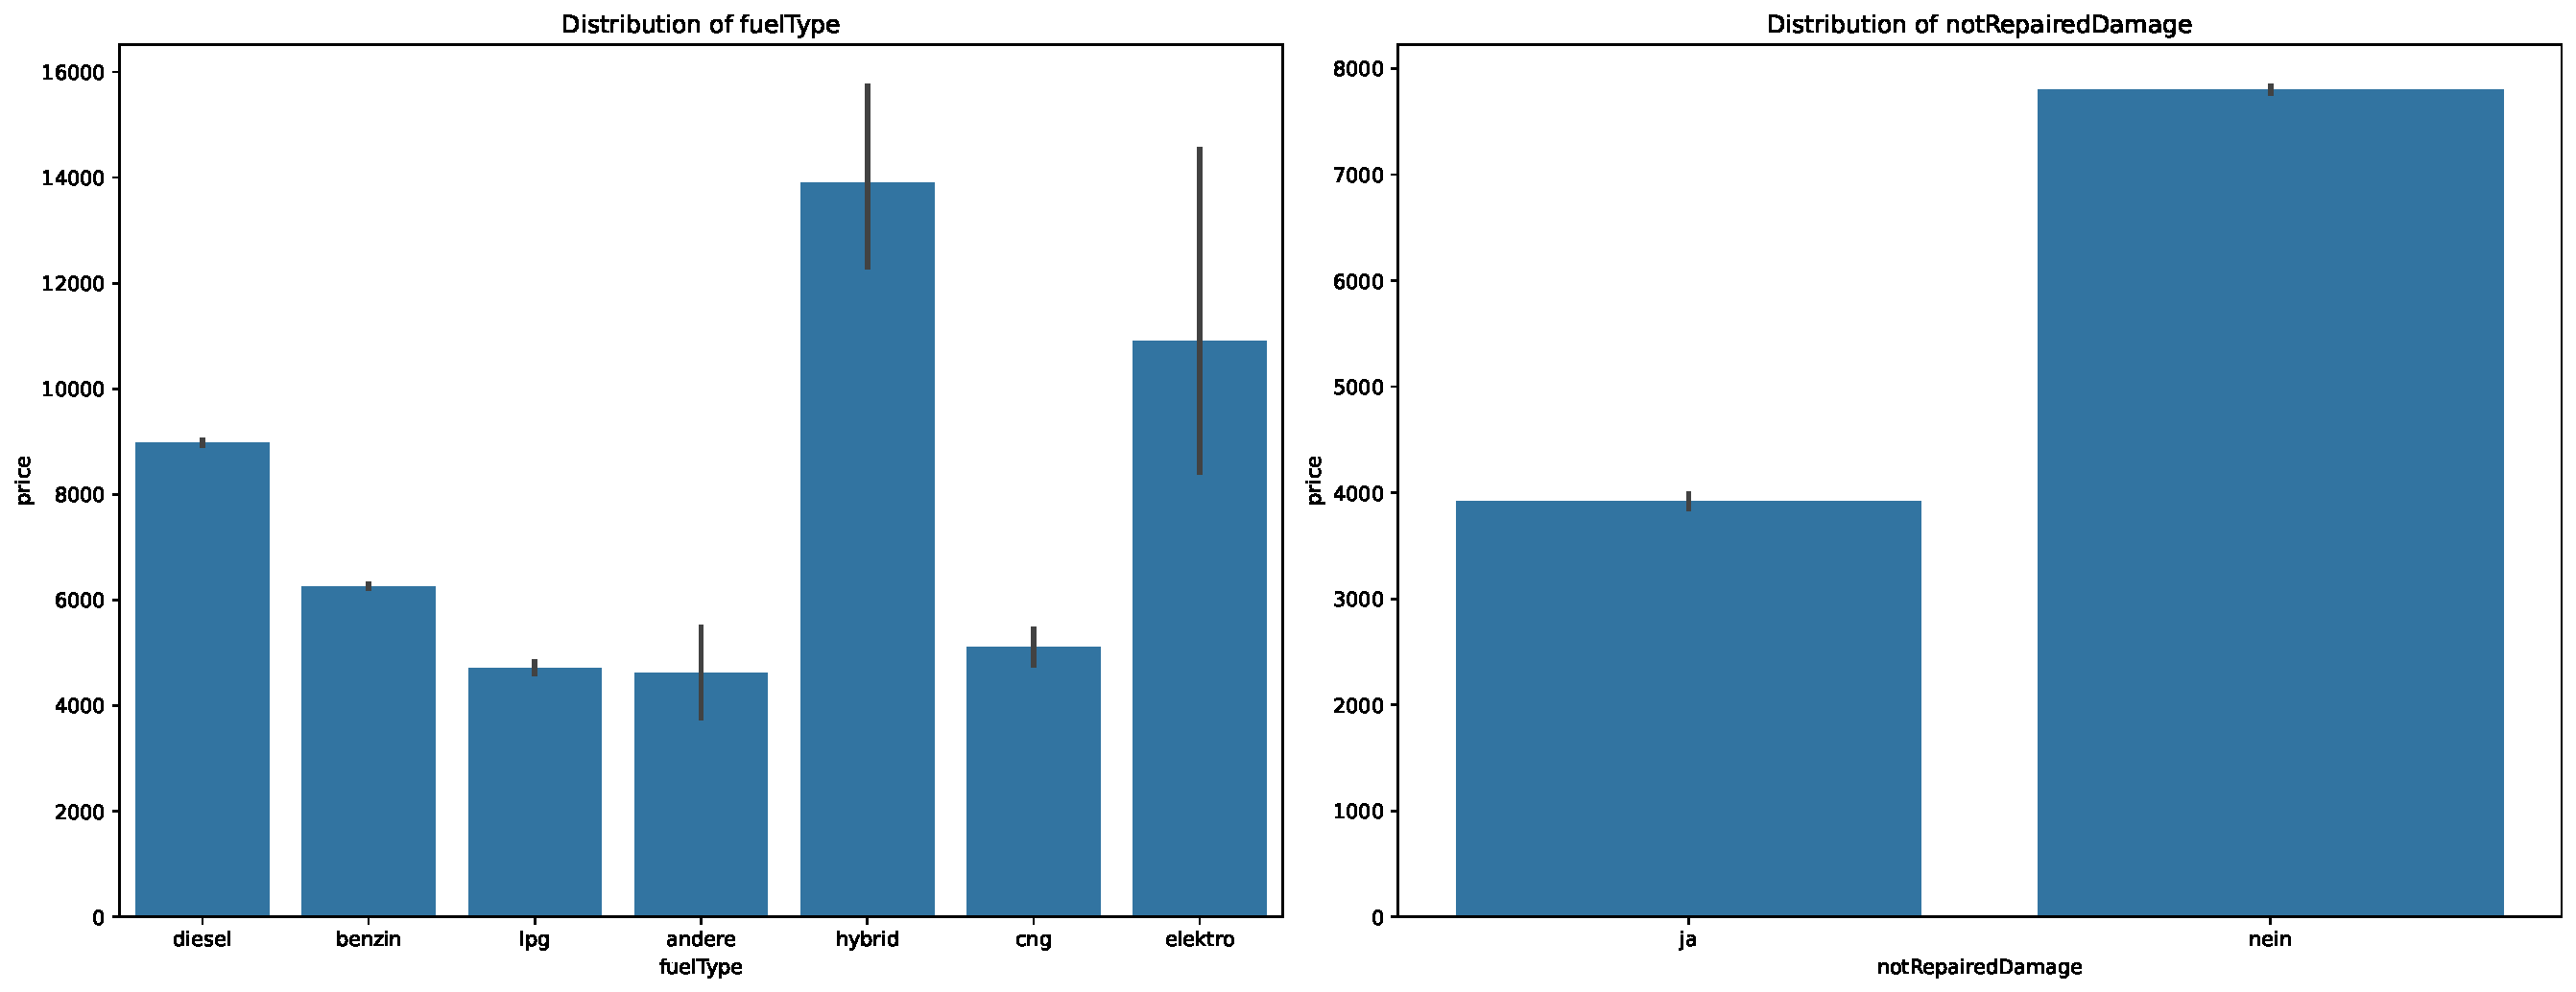
\includegraphics[scale=0.22]{cat_features_barplots2.pdf}
\end{frame}
\begin{frame}{Categorical Features Analysis}
        \center
        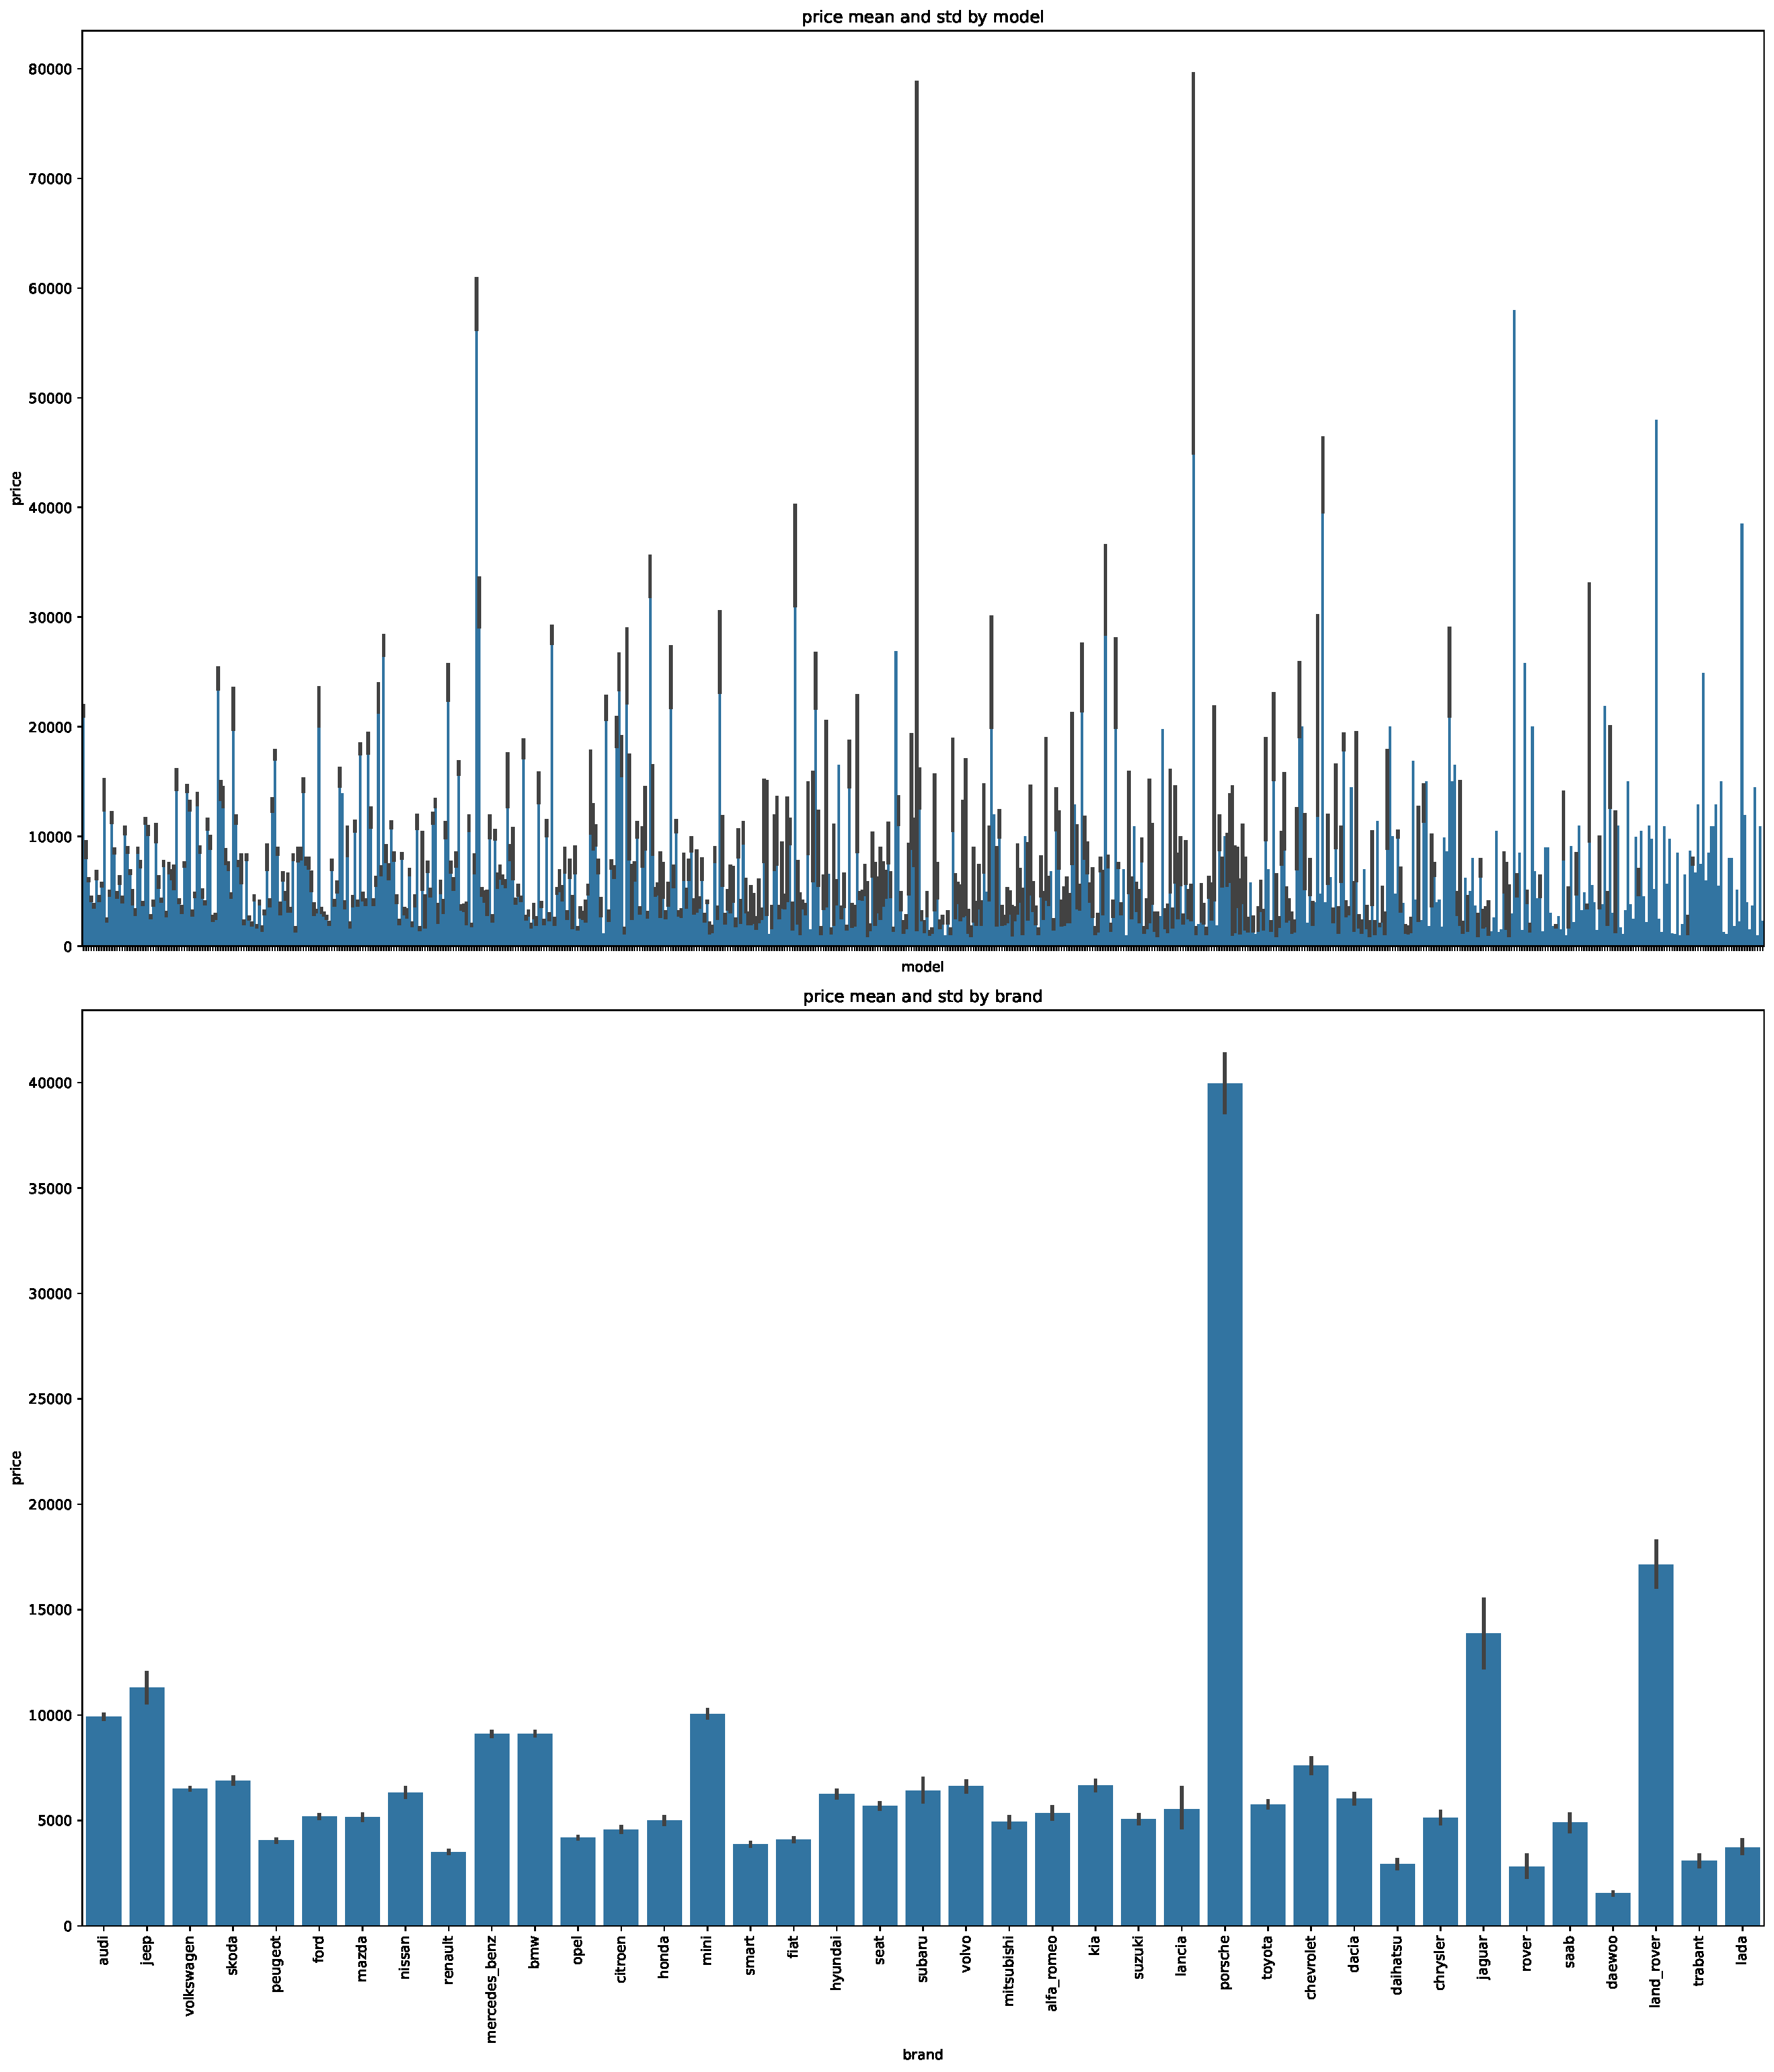
\includegraphics[scale=0.165]{model_brand_barplot.pdf}
\end{frame}

\begin{frame}{Categorical Features Analysis}
        \begin{itemize}
                \item Explored distributions of key categorical variables using
                        histograms.
                \item \textbf{ABtest (\texttt{abtest}):} Both categories
                        ("test" and "control") are similarly distributed, but
                        show no influence on price.
                \item \textbf{Vehicle Type (\texttt{vehicleType}):}
                        Distribution is dominated by a few types (kleinwagen,
                        limousine, kombi), which strongly influence price.
                \item \textbf{Gearbox (\texttt{gearbox}):} Majority are manual,
                        but automatic is also significant. Gearbox type shows
                        high correlation with price.
                \item \textbf{Month of Registration
                        (\texttt{monthOfRegistration}):} Mostly balanced,
                        except for "0" (likely missing values).
        \end{itemize}
\end{frame}

\begin{frame}{Categorical Features Analysis}
        \begin{itemize}
                \item \textbf{Fuel Type (\texttt{fuelType}):} Benzin dominates,
                        diesel also frequent. Rare types (lpg, andere, cng) can
                        be grouped as "other", but "hybrid" and "elektro" show
                        distinct price patterns.
                \item \textbf{Not Repaired Damage
                        (\texttt{notRepairedDamage}):} "Nein" dominates, but
                        "ja" shows much lower prices, indicating a strong
                        correlation with the target.
                \item \textbf{Model \& Brand:} Both have high correlation with
                        price and large within-category deviations, especially
                        for brands with many models (e.g., Porsche 911 vs
                        Cayenne).
                \item \textbf{General observations:}
                        \begin{itemize}
                                \item Many categorical features are unbalanced.
                                \item Outliers are present in every category.
                                \item Grouping or discarding rare categories
                                        considered to improve model stability.
                        \end{itemize}
        \end{itemize}
\end{frame}


\begin{frame}{Numerical Features Analysis for All Values}
        \center
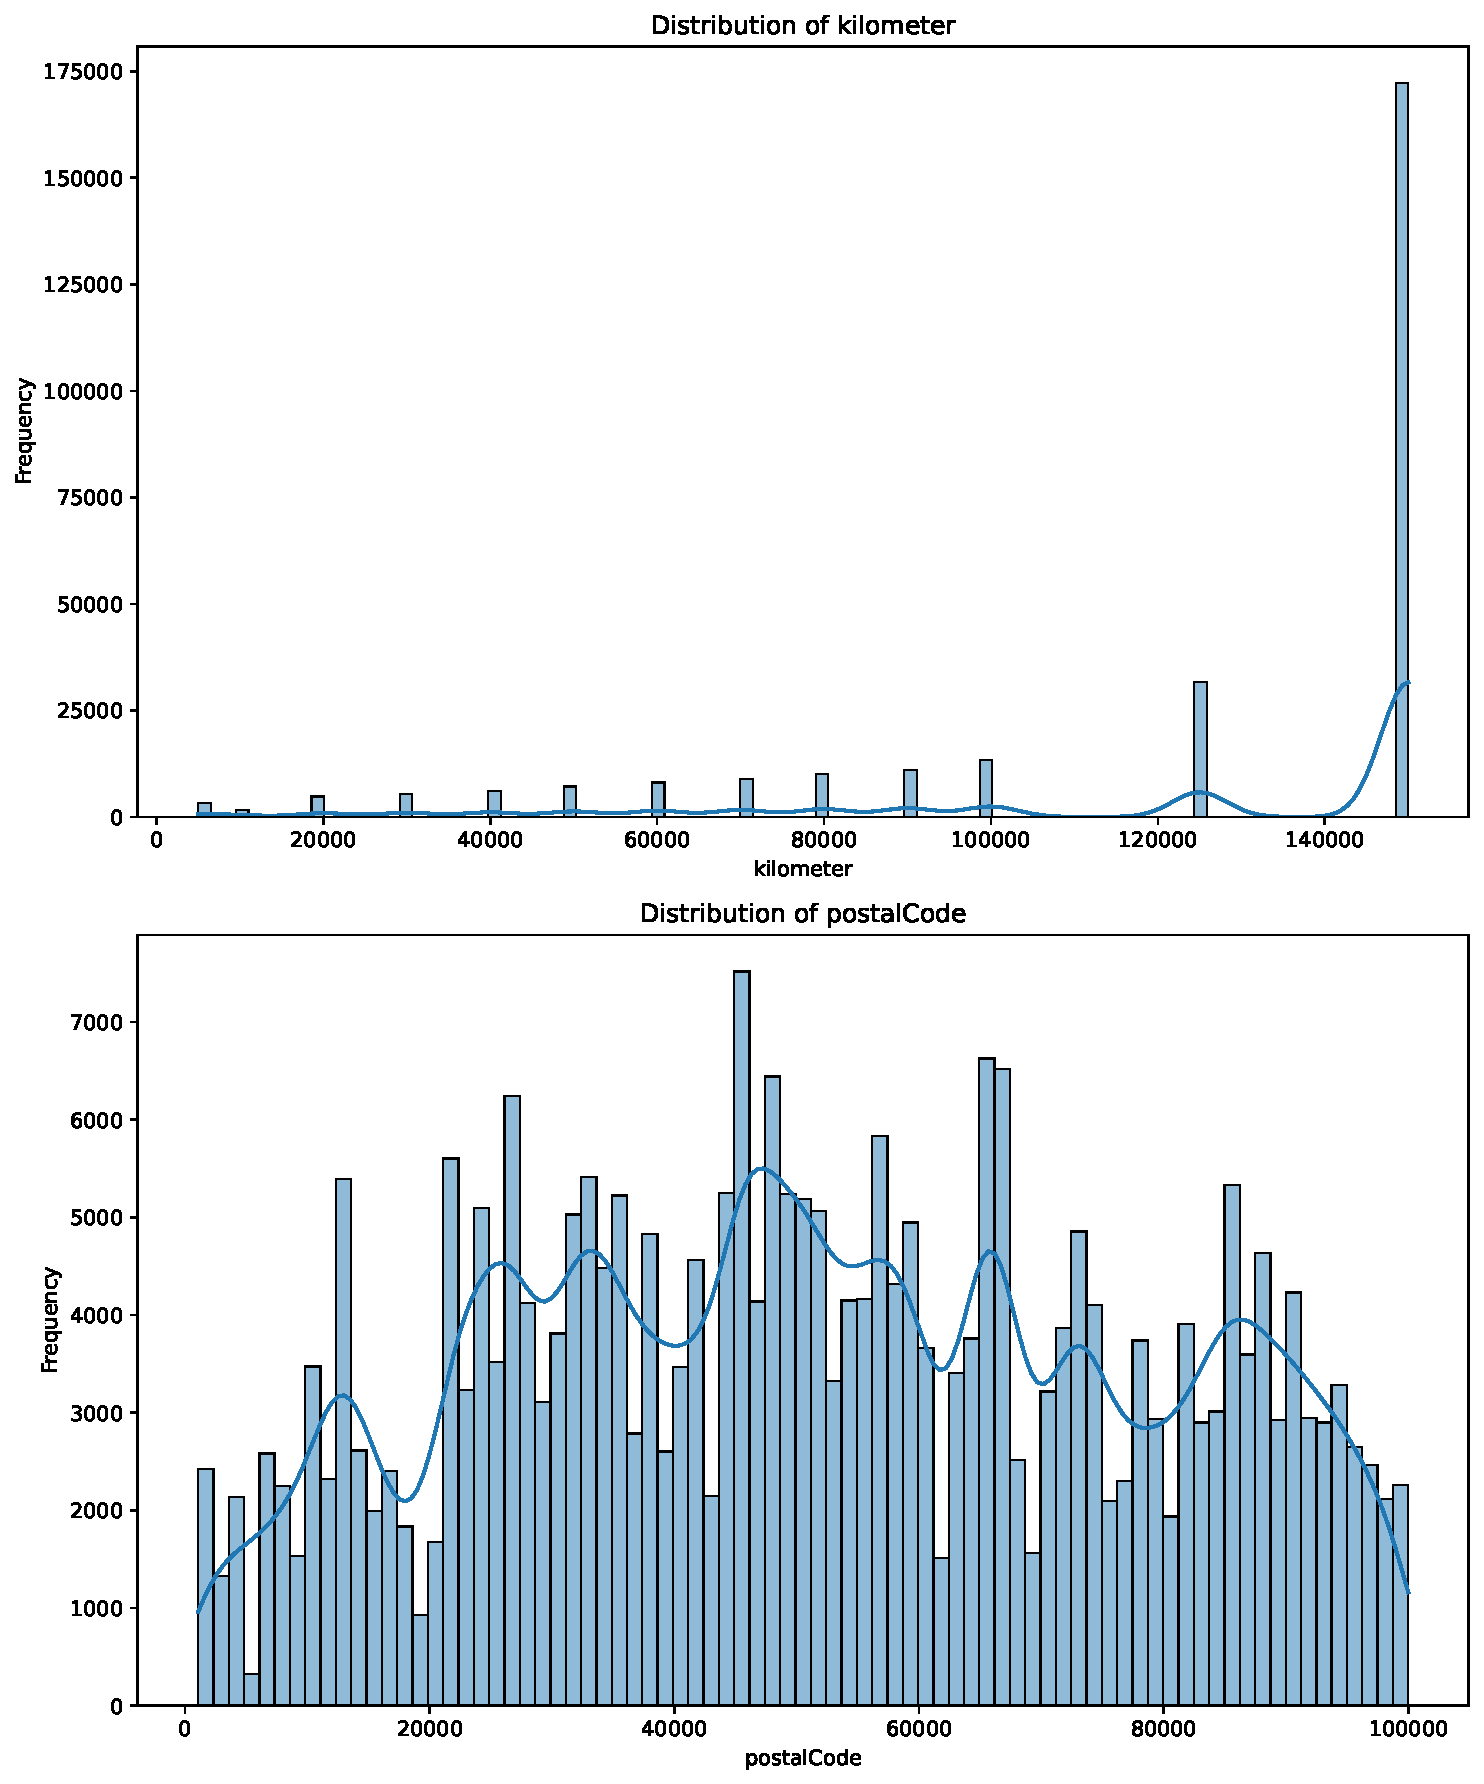
\includegraphics[scale=0.28]{kilometer_postalCode_distribution.pdf}
\end{frame}

\begin{frame}{Numerical Features Analysis for All Values}
        \center
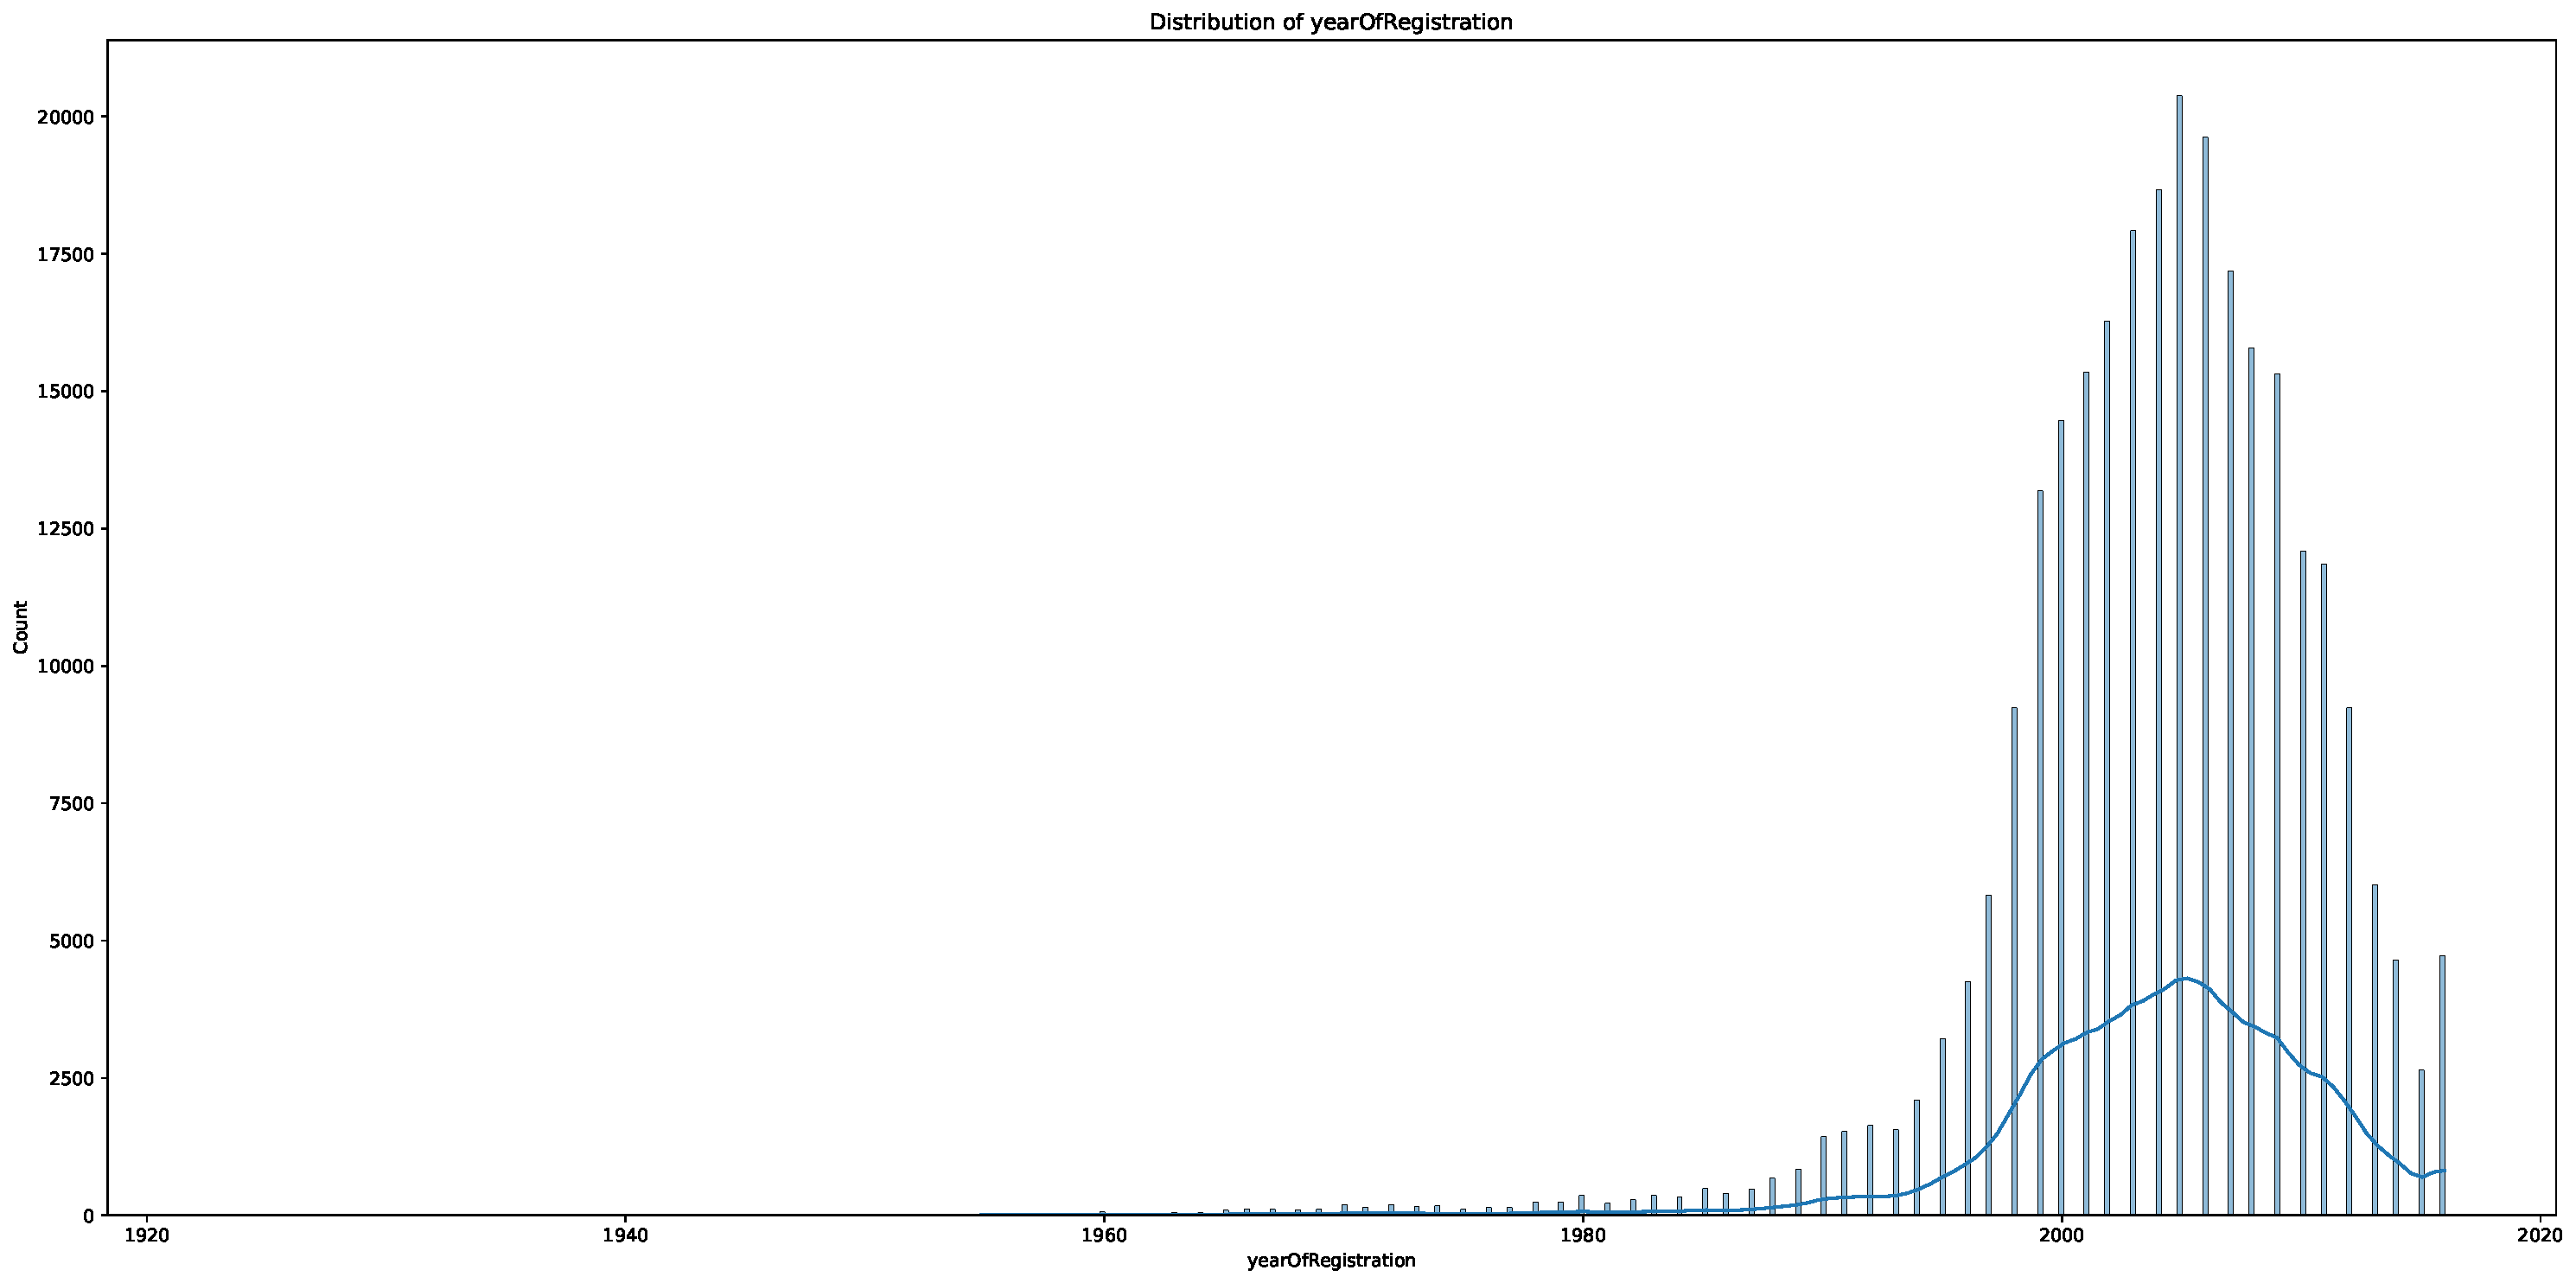
\includegraphics[scale=0.2]{yearOfRegistration_distribution.pdf}
\end{frame}

\begin{frame}{Numerical Features Analysis for All Values}
        \center
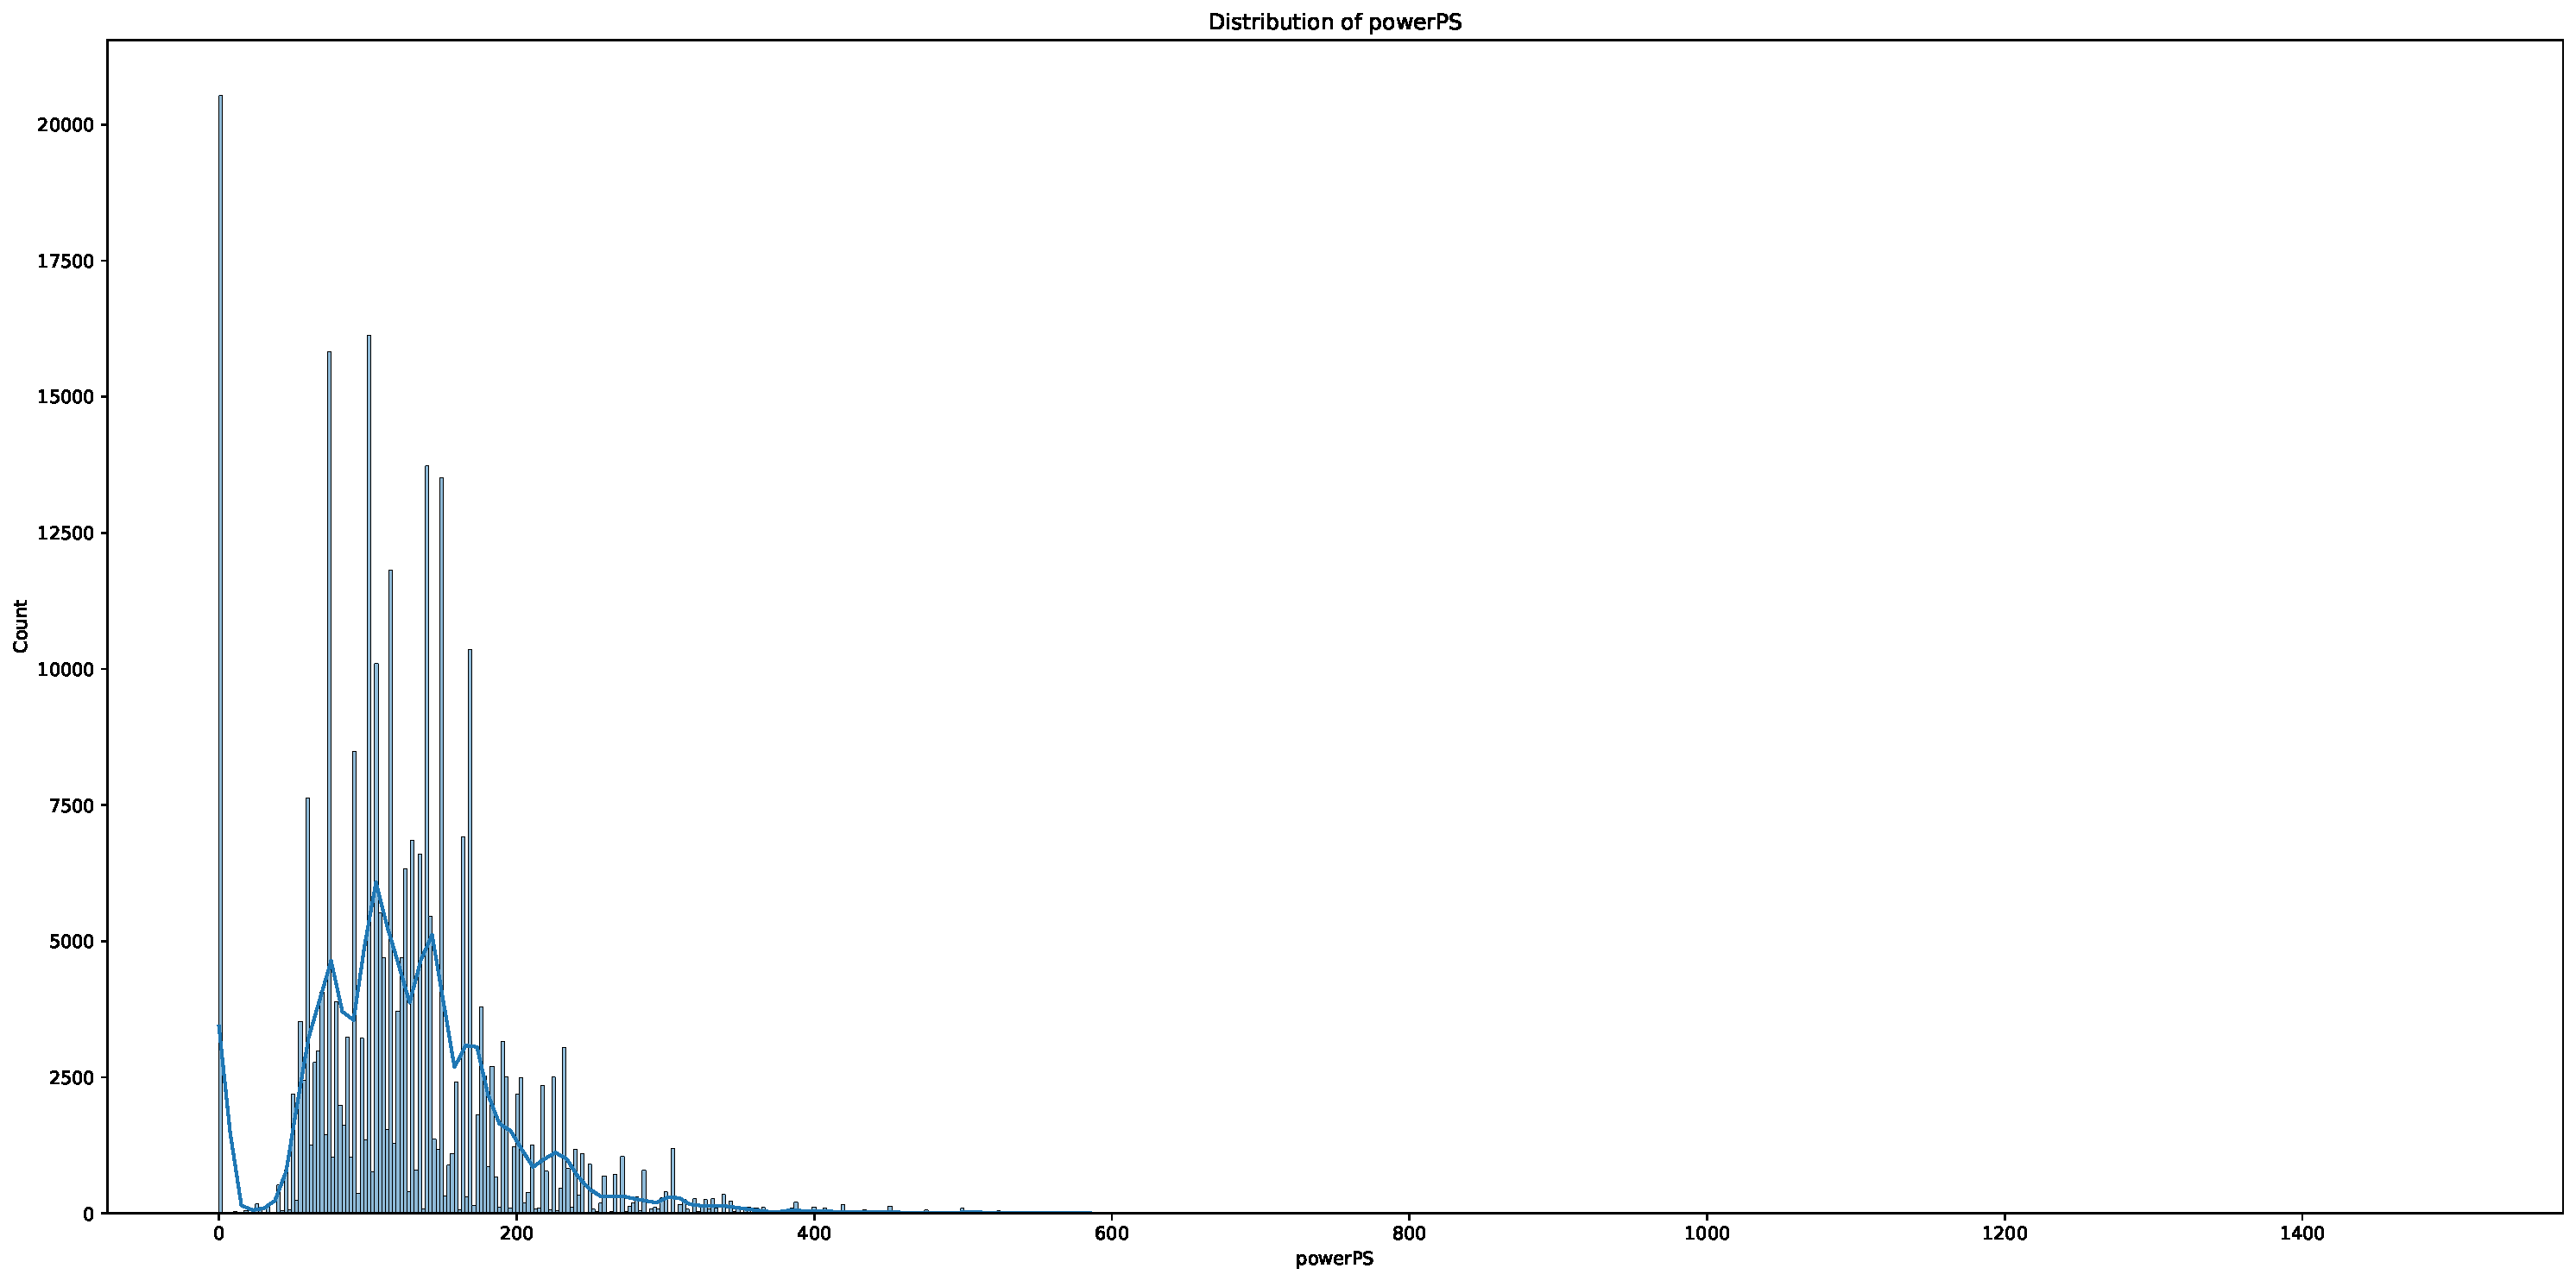
\includegraphics[scale=0.2]{powerPS_distribution.pdf}
\end{frame}

\begin{frame}{Numerical Features Analysis for All Values}
        \begin{itemize}
                \item Initial analysis revealed extreme skewness and
                        non-normality in several numerical features:
                        \begin{itemize}
                                \item \texttt{yearOfRegistration}: Skewness
                                        106.79
                                \item \texttt{powerPS}: Skewness 61.90 
                                \item \texttt{kilometer}: Skewness -1.33
                                \item \texttt{postalCode}: Skewness $\approx$
                                        0.02, no strong skew
                        \end{itemize}
                \item \textbf{Normality tests:} All tests (Anderson-Darling,
                        Kolmogorov-Smirnov, etc.) strongly rejected the
                        hypothesis of normal distribution for all features.
        \end{itemize}
\end{frame}

\begin{frame}{Numerical Features Analysis for Valid Values}
        \begin{itemize}
                \item After our initial analysis, we carefully checked each feature for valid value ranges:
                        \begin{itemize}
                                \item For \texttt{yearOfRegistration}, we kept
                                        only values from 1920 to 2016, since
                                        \texttt{DateCreated} was never after
                                        2016 and earlier years were invalid.
                                \item For \texttt{powerPS}, we kept only values
                                        less than or equal to 1500, as it is
                                        not realistic for a car under €200,000
                                        to have more power.
                                \item For \texttt{kilometer} and
                                        \texttt{postalCode}, we confirmed all
                                        values were within realistic ranges.
                        \end{itemize}
                \item This cleaning significantly reduced skewness:
                        \begin{itemize}
                                \item \texttt{yearOfRegistration}: -1.65
                                \item \texttt{powerPS}: 2.79
                                \item \texttt{kilometer}: -1.27
                                \item \texttt{postalCode}: $\approx$ 0
                        \end{itemize}
        \end{itemize}
\end{frame}

\begin{frame}{Correlation Analysis}
        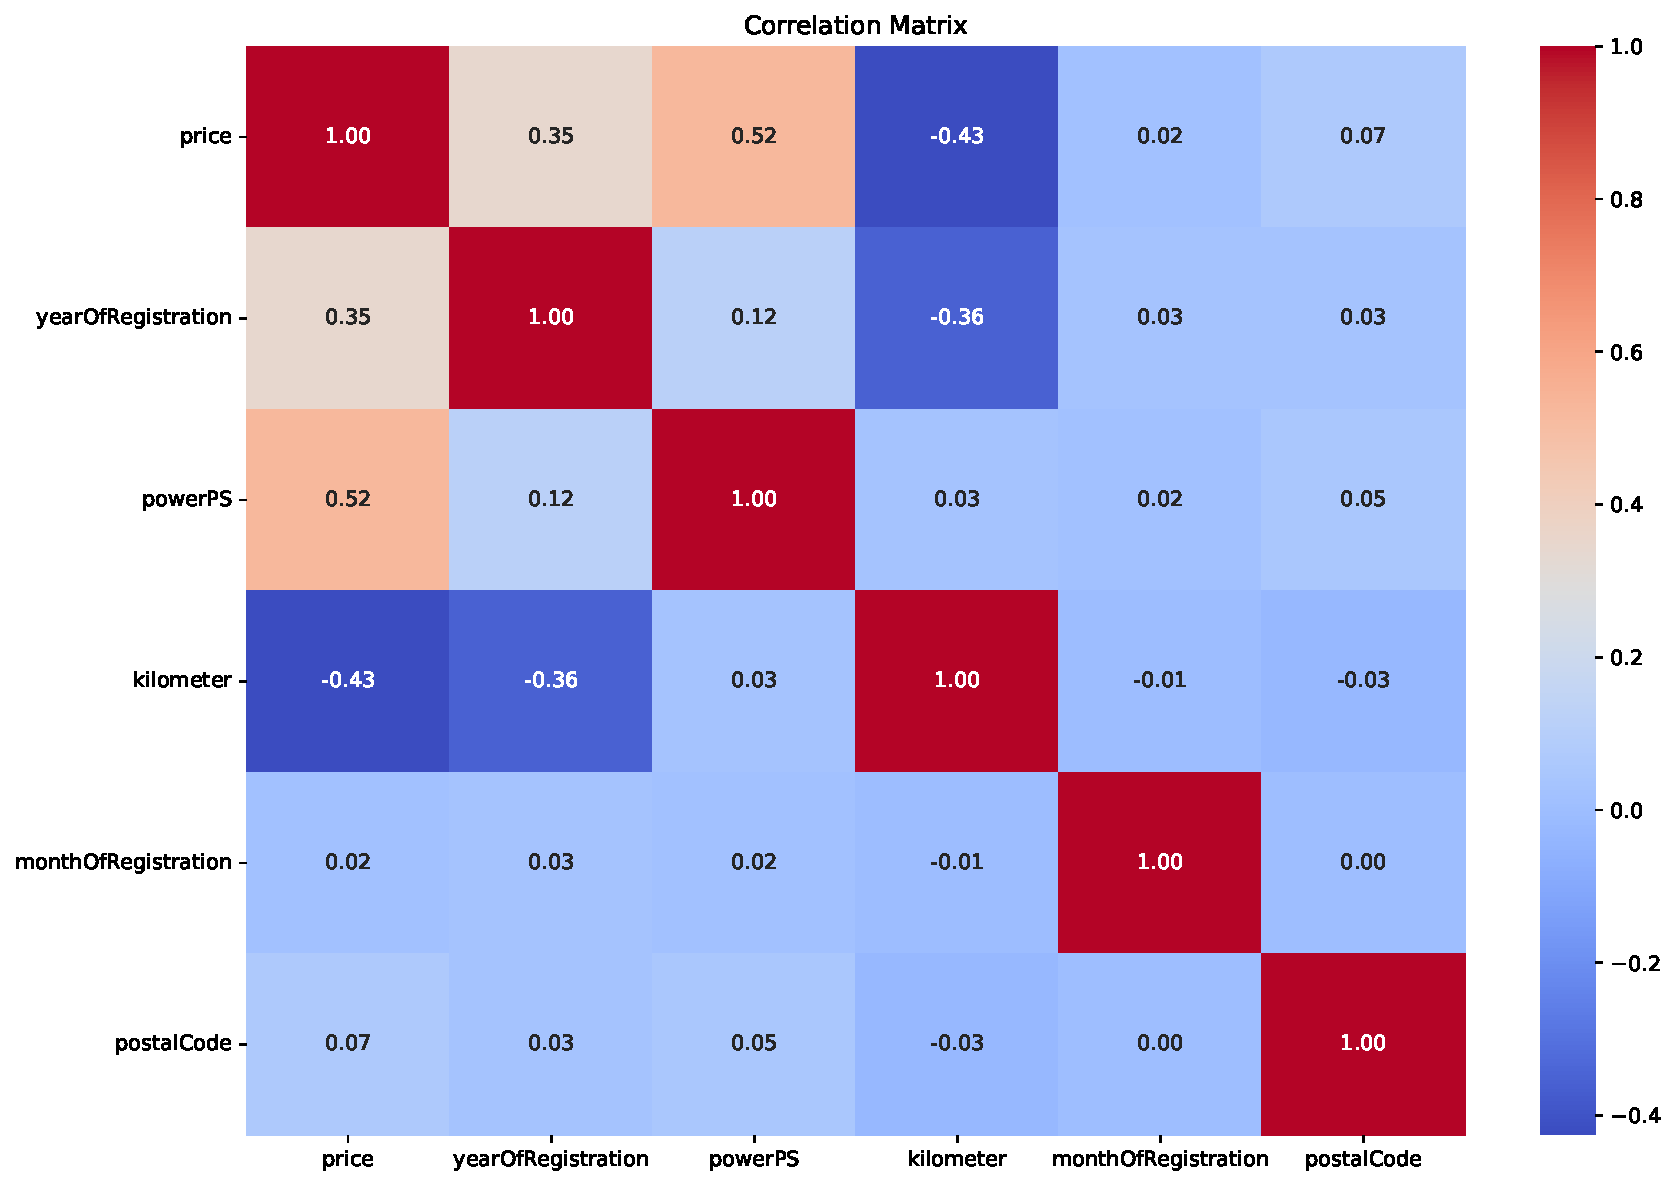
\includegraphics[scale=0.35]{heatmap.pdf}
\end{frame}

\begin{frame}{Correlation Analysis}
        \begin{itemize}
                \item \textbf{kilometer} and \textbf{price} have a moderate
                        negative correlation: cars with more kilometers tend to
                        be less expensive.
                \item \textbf{powerPS} and \textbf{price} have a moderate
                        positive correlation: higher power typically means a
                        higher price.
                \item \textbf{yearOfRegistration} and \textbf{price} have a
                        moderate positive correlation: newer cars are generally
                        more expensive.
                \item \textbf{yearOfRegistration} is negatively correlated with
                        \textbf{kilometer}: newer cars generally have lower
                        mileage.
                \item \textbf{postalCode} shows little or no correlation with
                        price, indicating it may not be a useful predictor.
                \item These correlations align with expectations and support
                        feature selection for modeling.
        \end{itemize}
\end{frame}

% Splitting Data
\section{Data Splitting}
\begin{frame}{Data Cleaning}
        \begin{itemize}
                \item \textbf{Set invalid values to missing:}
                        \begin{itemize}
                                \item \texttt{yearOfRegistration}: Years $<$
                                        1920 and $>$ 2016 are not realistic for
                                        used cars in our dataset. Setting these
                                        to NaN ensures we only use plausible
                                        registration years for modeling.
                                \item \texttt{powerPS}: Values below 4.5 or
                                        above 1500 are outside the range for
                                        real vehicles (especially considering
                                        our price limits). Marking these as
                                        missing, removes obvious errors and
                                        extreme outliers.
                                \item \texttt{monthOfRegistration}: A value of
                                        0 is not a valid month and likely
                                        indicates missing or unknown data, so
                                        we treat it as NaN.
                        \end{itemize}
                \item \textbf{Grouped rare \texttt{fuelType} categories:}
                        \begin{itemize}
                                \item Categories like "lpg" and "cng" had very
                                        few entries, making it hard for the
                                        model to learn about them.
                                \item We combined these into "andere" ("other")
                                        to improve statistical reliability.
                                \item "hybrid" and "elektro" were kept separate
                                        despite being rare, as they showed
                                        distinct price patterns and might be
                                        important for predictions.
                        \end{itemize}
        \end{itemize}
\end{frame}

\begin{frame}{Feature Engineering: Age Columns}
        \begin{itemize}
                \item Added two new features:
                        \begin{itemize}
                                \justifying
                                        \vspace{0.25em}
                                \item \texttt{adLifespan}: Time (in days)
                                        between when an ad was first seen and
                                        last seen. We now know how long it took
                                        for the car to be sold. It’s likely
                                        that its higher priced counterparts
                                        tend to remain listed longer than
                                        cheaper listings which quickly
                                        disappear after being seen often enough
                                        by members in related markets searching
                                        those platforms for new vehicles up for
                                        sale at any given time within certain
                                        parameters established such as location
                                        or age amongst others.
                                        \vspace{0.25em}
                                \item \texttt{carAge}: Age of the car in days
                                        at the time the ad was created.
                        \end{itemize}
        \end{itemize}
\end{frame}

\begin{frame}{Feature Engineering: Age Columns}
        \begin{itemize}
                \item Replaced date columns with these new features for
                        modeling convenience.
                \item Checked and corrected for negative or zero values in
                        \texttt{carAge}.
                \item Dropped columns: \texttt{registrationDate},
                        \texttt{dateCrawled}, \texttt{dateCreated},
                        \texttt{lastSeen}.
                \item \texttt{adLifespan} remained slightly right-skewed
                        (skewness: 0.96) and did not follow a normal
                        distribution.
                \item \texttt{carAge} and \texttt{yearOfRegistration} had a
                        perfect negative correlation ($r = -1.00$), so we
                        dropped \texttt{yearOfRegistration}.
        \end{itemize}
\end{frame}

\begin{frame}{Train/Test Split and Handling Imbalance}
        \begin{itemize}
                \item Split the dataset into train and test sets (80/20 split).
                \item Rare categories in \texttt{fuelType} ("hybrid" and
                        "elektro") were oversampled in the training set (20x)
                        to address class imbalance and ensure the model learns
                        from these cases (done after data splitting to avoid
                        leakage).
                \item After oversampling, shuffled the training set to mix
                        synthetic and real rows.
        \end{itemize}
\end{frame}

\begin{frame}{Scaling and Target Transformation}
        \begin{itemize}
                \item Applied robust scaling to numerical features and checked
                        their standard deviation:
                        \begin{itemize}
                                \item \texttt{carAge}: 0.864884
                                \item \texttt{powerPS}: 0.886468
                                \item \texttt{kilometer}: 0.809288
                                \item \texttt{adLifespan}: 0.760899
                        \end{itemize}
                \item They have high \texttt{std} which is what we wanted.
                \item Transformed the target variable (\texttt{price}) using
                        Box-Cox, as all values were positive, to reduce
                        skewness and improve model performance.
        \end{itemize}
\end{frame}

\section{Data Preprocessing}

\begin{frame}{Handling Missing Models Values}
\begin{table}[H]
\centering
\resizebox{\linewidth}{!}{%
\begin{tabular}{lll}
\toprule
name & model & brand \\
\midrule
Golf\_3\_1.6 & golf & volkswagen \\
A5\_Sportback\_2.7\_Tdi & NaN & audi \\
Jeep\_Grand\_Cherokee\_"Overland" & grand & jeep \\
GOLF\_4\_1\_4\_\_3TÜRER & golf & volkswagen \\
Skoda\_Fabia\_1.4\_TDI\_PD\_Classic & fabia & skoda \\
BMW\_316i\_\_\_e36\_Limousine\_\_\_Bastlerfahrzeug\_\_Export & 3er & bmw \\
Peugeot\_206\_CC\_110\_Platinum & 2\_reihe & peugeot \\
VW\_Derby\_Bj\_80\_\_Scheunenfund & andere & volkswagen \\
Ford\_C\_\_\_Max\_Titanium\_1\_0\_L\_EcoBoost & c\_max & ford \\
VW\_Golf\_4\_5\_tuerig\_zu\_verkaufen\_mit\_Anhaengerkupplung & golf & volkswagen \\
\bottomrule
\end{tabular}
}
\caption{Sample of car name, model, and brand from dataset}
\label{tab:car_name}
\end{table}
\end{frame}

\begin{frame}{Handling Missing Models Values}
        \begin{itemize}
                \item The \texttt{model} column contained many missing values,
                        making it unreliable for use directly.
                \item The \texttt{name} column, though messy and user-entered,
                        always existed and typically included the brand, model,
                        and extra info.
                \item \textbf{Solution:} We extracted the car model from the
                        \texttt{name} field using the following steps:
                        \begin{itemize}
                                \item Collected a comprehensive list of car
                                        brands and their possible models from
                                        the web.
                                \item Cleaned and tokenized the name, then
                                        generated all 1–3 word n-grams.
                                \item Matched these n-grams against known
                                        models for that brand using fuzzy
                                        matching.
                                \item If a strong match was found (above a
                                        similarity threshold), we filled in the
                                        missing \texttt{model}.
                        \end{itemize}
        \end{itemize}
\end{frame}

\begin{frame}{Results of Model Extraction}
        \begin{itemize}
                \item \textbf{Before extraction:} 12,148 missing values in the
                        \texttt{model} column.
                \item Using n-gram and fuzzy matching based on the car brand
                        and name, we reduced this to 4,114 missing values.
                \item \textbf{Limitations:}
                        \begin{itemize}
                                \item 2,857 entries could not be filled because
                                        the brand was \texttt{sonstige\_autos}
                                        (“other cars”).
                                \item 1,257 entries had insufficient
                                        information in the \texttt{name} field.
                        \end{itemize}
                \item \textbf{Final step:} To ensure data quality, we dropped
                        all rows where the \texttt{model} value remained
                        missing.
                \item This resulted in a clean and consistent dataset for
                        further analysis and modeling.
        \end{itemize}
\end{frame}

\begin{frame}{Feature Selection and Dimensionality Reduction}
        \begin{itemize}
                \item \textbf{Sequential Forward Selection (SFS):}
                        \begin{itemize}
                                \item Used SFS with XGBoost to select the most
                                        predictive features.
                                \item Best feature set: vehicleType, gearbox,
                                        powerPS, model, kilometer, fuelType,
                                        brand, notRepairedDamage, adLifespan,
                                        carAge.
                                \item Features \texttt{postalCode} and
                                        \texttt{monthOfRegistration} were not
                                        selected, confirming their low
                                        predictive value.
                        \end{itemize}
                \item \textbf{Extra Trees Classifier:}
                        \begin{itemize}
                                \item Attempted to compute feature importance.
                                \item Kernel repeatedly crashed with larger
                                        \texttt{n\_estimators}, so results are
                                        unstable and not reliable for ranking.
                        \end{itemize}
                \item \textbf{Dimensionality Reduction:}
                        \begin{itemize}
                                \item \textbf{PCA} not used: only suitable for
                                        continuous numerical data, but our
                                        dataset contains many categorical
                                        variables.
                                \item \textbf{SVD} not used: most effective for
                                        large, sparse matrices, which does not
                                        apply here.
                                \item Not a limitation, as we do not have too
                                        many features.
                        \end{itemize}
        \end{itemize}
\end{frame}

\begin{frame}{Feature Selection}
        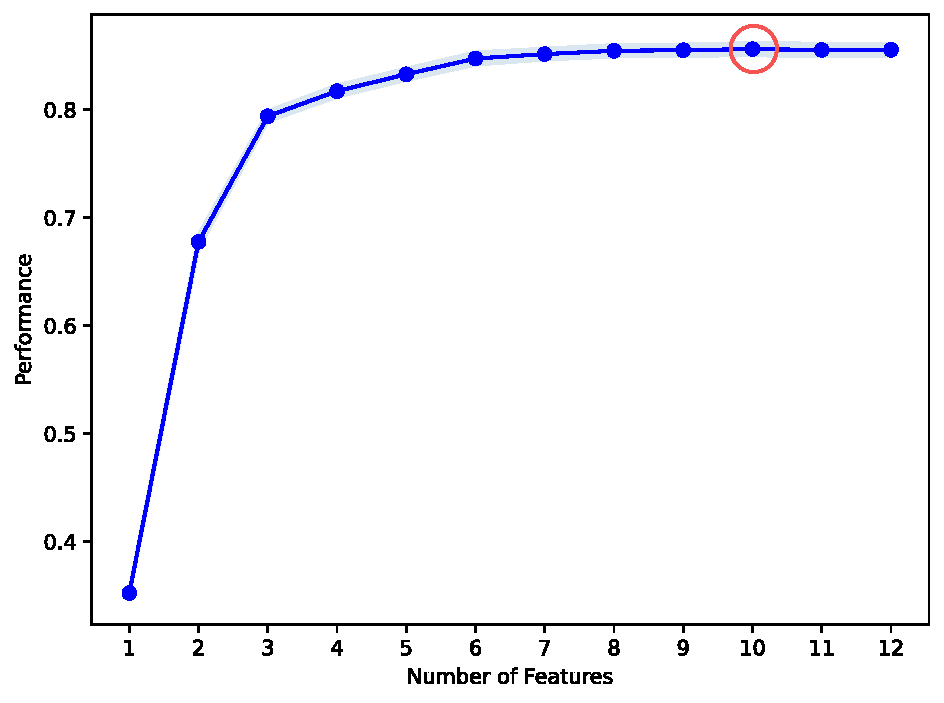
\includegraphics[width=\linewidth]{sfs.pdf}
\end{frame}

\begin{frame}{Dataset Versions and Preprocessing Strategies}
        \begin{itemize}
                \item Created multiple dataset versions (V1–V8) to explore the
                        impact of different preprocessing strategies:
                        \begin{itemize}
                                \item Imputation strategies: mean, most
                                        frequent, iterative.
                                \item Encoding methods: label encoding, one-hot
                                        encoding.
                                \item Skewness correction: Box-Cox,
                                        Yeo-Johnson.
                                \item Scaling: RobustScaler, MinMaxScaler.
                                \item Normalization: normalized whole rows with
                                        \texttt{l2}
                                \item Compared full feature sets and subsets
                                        selected by SFS.
                        \end{itemize}
                \item These experiments allowed us to identify the best
                        preprocessing pipeline for optimal model performance.
        \end{itemize}
\end{frame}

\section{Model Training and Evaluation}
\begin{frame}{Model Training and Evaluation}
    \begin{itemize}
        \item Trained and compared six regression models (Random Forest,
                AdaBoost, XGBoost, CatBoost, KNN, Decision Tree) using 10-fold
                cross-validation.
        \item Compared each model across all dataset and target versions
                (original and unskewed).
        \item \textbf{Top-performing algorithms:}
        \begin{itemize}
            \item CatBoost (\textbf{original target}): $R^2 = 0.856$
            \item RandomForest (\textbf{unskewed target}): $R^2 = 0.853$
        \end{itemize}
        \item \textbf{Best dataset versions:}
        \begin{itemize}
            \item V7 (unskewed target): $R^2 = 0.777$
            \item V8 (unskewed target): $R^2 = 0.776$
        \end{itemize}
    \end{itemize}
\end{frame}

\begin{frame}{Best Dataset Versions}
        \begin{itemize}
                \item \textbf{Version V7:}
                        \begin{itemize}
                                \item Used the optimal feature subset selected
                                        by Sequential Forward Selection (SFS).
                                \item Applied mean imputation for numerical
                                        features and most frequent imputation
                                        for categorical features.
                                \item Encoded categorical features with label
                                        encoding.
                                \item Scaled numerical features using
                                        RobustScaler.
                        \end{itemize}
                \item \textbf{Version V8:}
                        \begin{itemize}
                                \item Built on V7 preprocessing steps.
                                \item Additionally applied Yeo-Johnson power
                                        transformation to unskew key numerical
                                        features: \texttt{kilometer},
                                        \texttt{carAge}, \texttt{powerPS},
                                        \texttt{adLifespan}.
                        \end{itemize}
        \end{itemize}
\end{frame}

\begin{frame}{Hyperparameter Tuning}
    \begin{itemize}
        \item After identifying the best-performing algorithms and dataset
                version, we applied \textbf{GridSearchCV} to tune
                hyperparameters and evaluate model performance using the $R^2$
                score.
        \item However, for values \texttt{cv}~\textgreater~2 the OS killed our
                process for using too much memory (\texttt{google collab} also
                killed our process for taking way too long, both for CPU and
                GPU).
        \item \textbf{Final results:}
        \begin{itemize}
            \item The best overall model was \textbf{CatBoost} on dataset
                    \textbf{V8}, unskewed, which achieved an $R^2$ score of
                    \textbf{0.853} on the test set and \textbf{0.876} on the
                    training set.
            \item The best version of \textbf{RandomForest} on dataset
                    \textbf{V8}, unskewed, achieved an $R^2$ score of
                    \textbf{0.835} on the test set and \textbf{0.976} on the
                    training set.
        \end{itemize}
        \item CatBoost showed strong generalization with no significant
                overfitting. However, RandomForest seems to have been
                overtrained.
        \item CatBoost slightly outperformed RandomForest in the final
                evaluation.
    \end{itemize}
\end{frame}

\section{Classification Problem: Predicting Price Categories}
\begin{frame}
        \centering
        \Huge
        Turning Price Prediction Into a Classification Problem
\end{frame}

\begin{frame}{From Regression to Classification}
        \begin{itemize}
                \item In addition to regression, we transformed the problem
                        into classification by categorizing car prices.
                \item Used \texttt{pd.cut} to bin the continuous price into
                        four categories:
                        \begin{itemize}
                                \item low (\textless~€~5,000)
                                \item low average (€~5,000–10,000)
                                \item middle average (€~10,000–50,000)
                                \item high (\textgreater~€~50,000)
                        \end{itemize}
                \item This allows us to analyze model performance for distinct
                        price segments and understand price ranges better.
        \end{itemize}
\end{frame}

\begin{frame}{Data Preparation for Classification}
        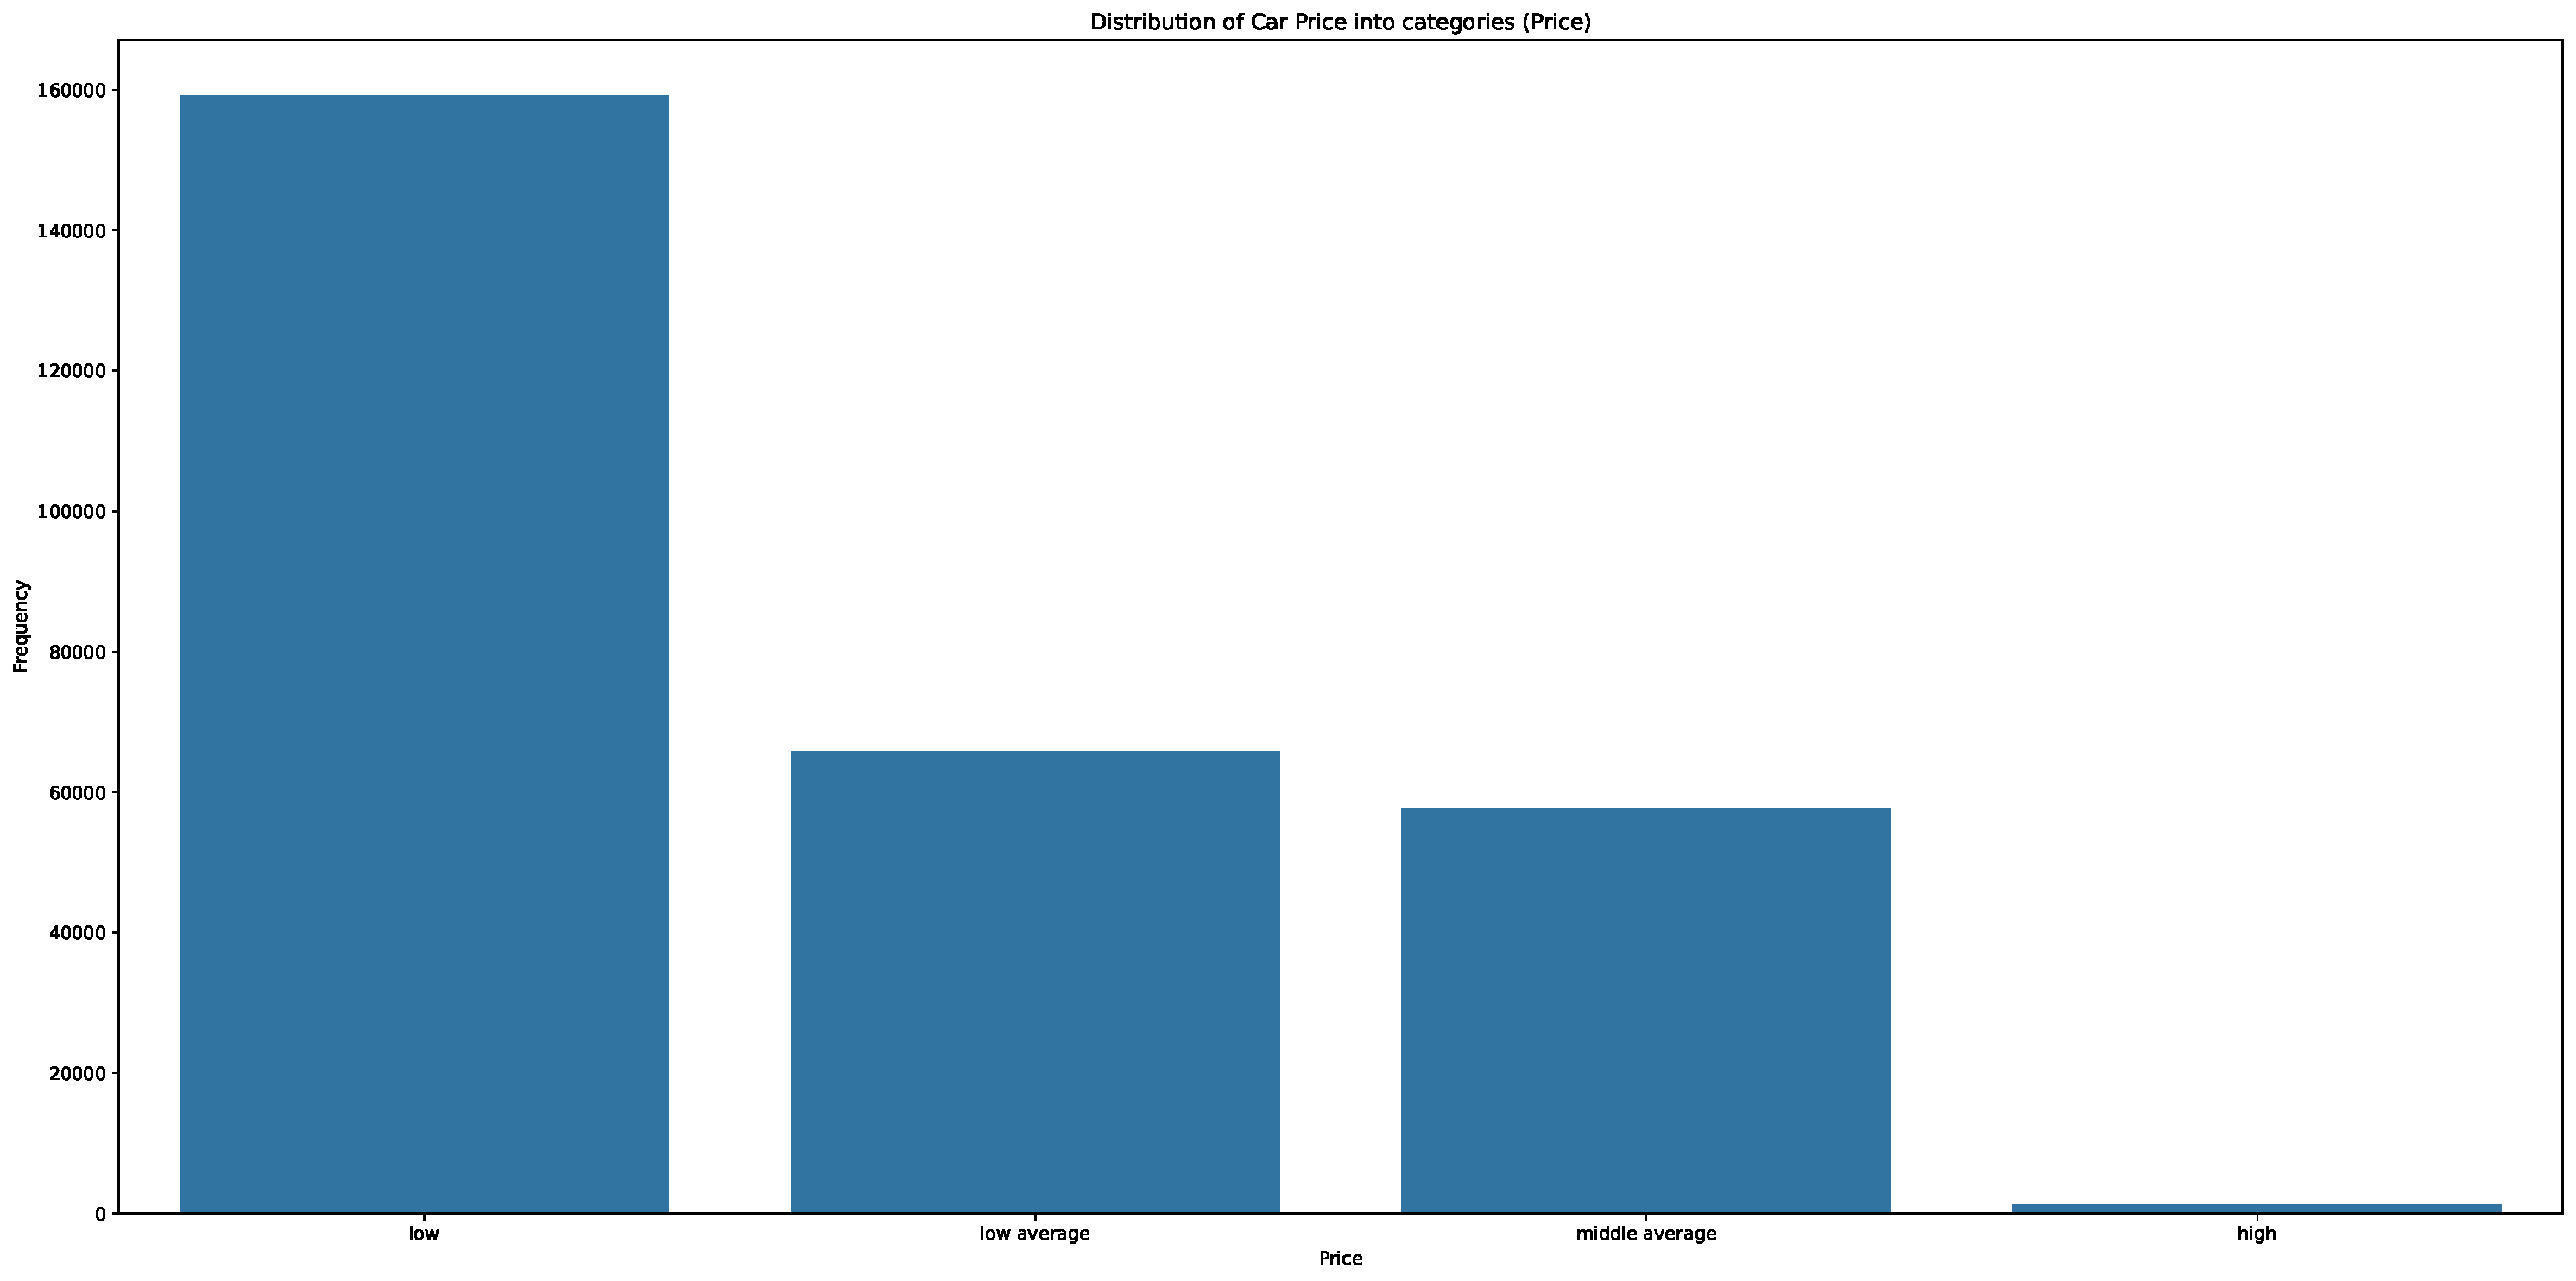
\includegraphics[width=\linewidth]{bins.pdf}
\end{frame}

\begin{frame}{Data Preparation for Classification}
        \begin{itemize}
                \item Dropped the original price column, used the new price
                        category as target.
                \item Performed an 80/20 train-test split before scaling or
                        encoding to avoid data leakage.
                \item Oversampled rare fuel types ("hybrid" and "elektro") in
                        the training set (20$\times$) to improve learning for
                        underrepresented categories.
                \item Created new dataset versions (V9, V10) using:
                        \begin{itemize}
                                \item Feature selection (from regression task).
                                \item Imputation for missing values.
                                \item One-hot encoding and dimensionality
                                        reduction (LDA) for categorical
                                        features.
                                \item Scaling and unskewing for numerical
                                        features.
                        \end{itemize}
        \end{itemize}
\end{frame}

\begin{frame}{Classification Models and Evaluation}
    \begin{itemize}
        \item Evaluated several classifiers with 10-fold cross-validation:
        \begin{itemize}
            \item RandomForest, XGBoost, CatBoost, DecisionTree, AdaBoost,
                    KNeighbors, Logistic Regression, GaussianNB
        \end{itemize}
        \item Used weighted F1-score as the main metric due to class imbalance.
        \item Hyperparameter tuning performed for the best pipelines
                (RandomForest, XGBoost) with GridSearchCV.
        \item \textbf{Best performing algorithms:}
        \begin{itemize}
            \item RandomForest: F1-score = \textbf{0.873}
            \item XGBoost: F1-score = \textbf{0.864}
        \end{itemize}
        \item \textbf{Best dataset versions:}
        \begin{itemize}
            \item V10: F1-score = \textbf{0.817}
            \item V8: F1-score = \textbf{0.811}
        \end{itemize}
    \end{itemize}
\end{frame}

\begin{frame}{Best Dataset Versions}
        \begin{itemize}
                \item \textbf{Version V8:}
                        \begin{itemize}
                                \item Used the optimal feature subset from
                                        Sequential Forward Selection (SFS).
                                \item Applied mean imputation to numerical
                                        features and most frequent imputation
                                        to categorical features.
                                \item Encoded categorical features with label
                                        (ordinal) encoding.
                                \item Scaled numerical features using
                                        RobustScaler.
                                \item Applied Yeo-Johnson power transformation
                                        to unskew \texttt{kilometer},
                                        \texttt{carAge}, \texttt{powerPS},
                                        \texttt{adLifespan}.
                        \end{itemize}
                \item \textbf{Version V10:}
                        \begin{itemize}
                                \item Used features selected from \texttt{SFS}.
                                \item Numerical features were imputed using the
                                        \texttt{mean} strategy.
                                \item Numerical features were scaled using 
                                        \texttt{RobustScaler}.
                                \item Applied one-hot encoding to categorical
                                        features, followed by \texttt{LDA} for
                                        dimensionality reduction.
                                \item Also applied \texttt{Yeo-Johnson} power
                                        transformation to unskew key numerical
                                        features.
                        \end{itemize}
        \end{itemize}
\end{frame}

\begin{frame}{Hyperparameter Tuning}
    \begin{itemize}
        \item After identifying the best-performing classification algorithms
                and dataset version, we applied \textbf{GridSearchCV} to tune
                hyperparameters and evaluated model performance using the
                weighted F1-score.
        \item However, for values \texttt{cv}~\textgreater~2 the OS killed our
                process for using too much memory (\texttt{google collab} also
                killed our process for taking way too long both for CPU and
                GPU).
        \item \textbf{Final results:}
        \begin{itemize}
            \item The best overall model was \textbf{XGBoostClassifier} on
                    dataset V8, which achieved a weighted F1-score of
                    \textbf{0.875} on the test set and \textbf{0.928} on the
                    training set.
            \item The best version of \textbf{RandomForestClassifier} on
                    dataset V8 achieved a weighted F1-score of \textbf{0.874}
                    on the test set and \textbf{0.976} on the training set.
            \item XGBoost showed strong generalization with no significant
                overfitting. However, RandomForest seems to have been
                overtrained.
            \item XGBoost slightly outperformed RandomForest in the final
                evaluation.
        \end{itemize}
    \end{itemize}
\end{frame}

\begin{frame}{Key Takeaways: Classification Task}
        \begin{itemize}
                \item Transforming price prediction to classification allowed
                        us to focus on distinct market segments.
                \item Proper binning, feature selection, dimensionality
                        reduction, and robust preprocessing are essential for
                        strong performance.
                \item RandomForest and XGBoost achieved the highest F1-scores,
                        showing strong capability for price category
                        prediction.
        \end{itemize}
\end{frame}

\begin{frame}
        \centering
        \Huge
        Thank you! \\
        Questions?
\end{frame}

\end{document}
